
\section{Metodología}
\textbf{SiteUp} ha seguido una metodología de desarrollo ágil en la que,
mediante fases de desarrollo rápidas y ligeras, se intenta evitar los formales
caminos de las metodologías tradicionales, enfocándose en las personas y
obteniendo así resultados en etapas más tempranas del desarrollo.

En las sucesivas secciones y capítulos se detallará el proceso de análisis y
posteriores fases del proyecto en la última iteración del proyecto. Así se
consigue una documentación más concisa y cercana al producto final.

\section{Modelo conceptual}

De acuerdo a lo reflejado en el apartado~\ref{sec:requisitos-informacion} se
presenta el diagrama~\ref{fig:modelo-conceptual} en el que se identifican las
clases, sus atributos y las relaciones entre ellas.

\begin{figure}[hp]
  \centering
  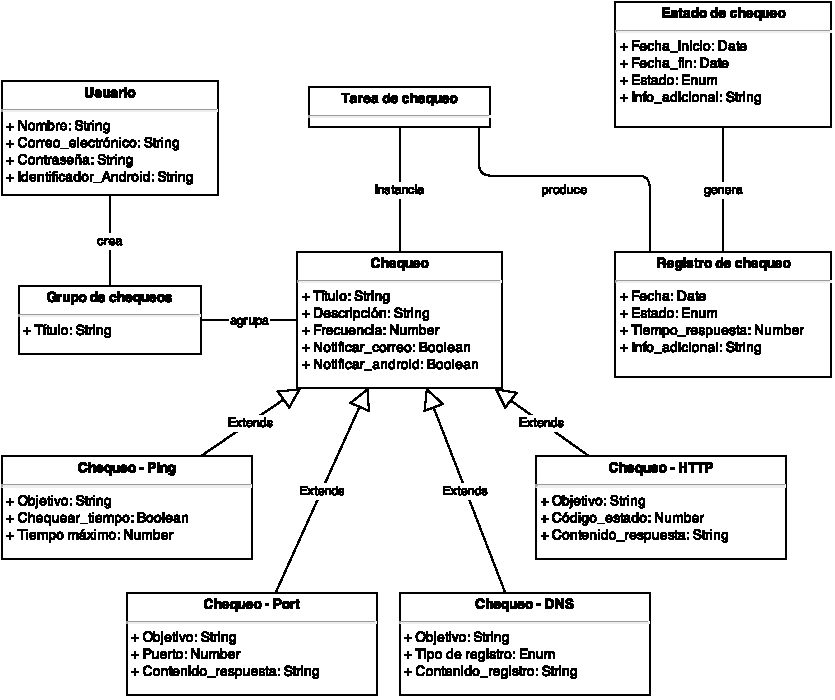
\includegraphics[width=\textwidth]{4_analisis/diagrama_clases_conceptuales}
  \caption{Modelo conceptual}
  \label{fig:modelo-conceptual}
\end{figure}


\subsection{Usuario}

\begin{description}
\item[Nombre] Nombre elegido por el usuario.
\item[Correo electrónico] Dirección de correo electrónico.
\item[Contraseña] Contraseña para el login del usuario.
\item[Identificador Android] Identificador único del dispositivo Android del usuario.
\end{description}

\subsection{Grupo de chequeos}

\begin{description}
\item[Título] Título para identificar al grupo de chequeos.
\end{description}

\subsection{Chequeo}

\begin{description}
\item[Título] Título para identificar al chequeo.
\item[Descripción] Información adicional en forma textual sobre el chequeo.
\item[Frecuencia de chequeo] Frecuencia temporal del chequeo, expresada en minutos.
\item[Notificar por correo] Indica si los cambios de estado del chequeo deben notificarse por correo electrónico.
\item[Notificar por Android] Indica si los cambios de estado del chequeo deben notificarse por la aplicación Android.
\end{description}

\subsection{Registro de chequeo}

\begin{description}
\item[Fecha] Fecha y hora en la que se obtuvo este registro.
\item[Estado] Resultado del lanzamiento del chequeo. El estado puede ser
  \textit{Up}, que indica que el objetivo está funcionando; \textit{Down}, que
  indica que el objetivo no está funcionando correctamente; y \textit{Error},
  que indica que hubo un problema lanzando el chequeo.
\item[Tiempo de respuesta] \textit{(solo para chequeos tipo Ping)} indica el
  tiempo de respuesta medio obtenido al lanzar el chequeo.
\item[Información adicional] Datos extra en caso de que el estado no sea \textit{Up}.
\end{description}

\subsection{Chequeo - Ping}

\begin{description}
\item[Objetivo] Identificador de la máquina a la que enviar el ping. Debe ser un
  \textit{hostname} o una IP.
\item[Chequear tiempo?] Indica si además de chequear que la máquina responde al
  ping, también se debe chequear que el tiempo de respuesta sea menor que el indicado.
\item[Tiempo máximo] Tiempo de respuesta máximo permitido.
\end{description}

\subsection{Chequeo - Port}

\begin{description}
\item[Objetivo] Identificador de la máquina a chequear.
\item[Puerto objetivo] Puerto remoto en la máquina que se chequeará.
\item[Contenido de respuesta] \textit{(opcional)} Cadena de caracteres que
  deberá estar presente en la respuesta obtenida de la máquina remota.
\end{description}

\subsection{Chequeo - DNS}

\begin{description}
\item[Objetivo] Dominio sobre el que realizar el chequeo de DNS.
\item[Tipo de registro] Tipo de registro DNS a verificar. Puede ser A, AAAA, CNAME, MX y TXT.
\item[Contenido de registro] El contenido que debe tener el registro a consultar.
\end{description}

\subsection{Chequeo - HTTP}

\begin{description}
\item[Objetivo] URL a verificar.
\item[Código de estado] Código que debe devolver la petición a la URL indicada.
\item[Cadena de respuesta] \textit{(opcional)} Cadena que debe encontrarse en la
  respuesta obtenida.
\end{description}



\section{Modelo de casos de uso}

\subsection{Actores}

En este apartado se describen los diversos roles que juegan los usuarios del
sistema. Se reflejan todos ellos en el diagrama \ref{fig:actores}.

\begin{figure}[h]
  \centering
  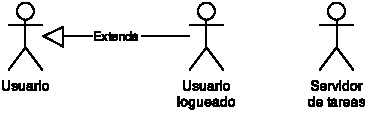
\includegraphics[width=0.7\textwidth]{4_analisis/diagrama_actores}
  \caption{Diagrama de actores}
  \label{fig:actores}
\end{figure}

\subsubsection{Usuario}

\begin{center}
  \begin{tabularx}{\textwidth}{|c|X|}
    \hline
     & Usuario \\

    \hline

    Descripción & Usuario libre de la aplicación, que puede haber hecho login previamente o no. \\

    \hline
  \end{tabularx}

\end{center}


\subsubsection{Usuario logueado}

\begin{center}
  \centering
  \begin{tabularx}{\textwidth}{|c|X|}
    \hline
     & Usuario logueado \\

    \hline

    Descripción & Usuario que previamente se ha registrado y ha hecho login en el sistema. \\

    \hline
  \end{tabularx}
\end{center}

\subsubsection{Servidor de tareas}

\begin{center}
  \centering
  \begin{tabularx}{\textwidth}{|c|X|}
    \hline
     & Servidor de tareas \\

    \hline

    Descripción & Servidor de tareas asíncronas que periódicamente lanza tareas que previamente se hayan dado de alta. \\

    \hline
  \end{tabularx}
\end{center}

\subsection{Subsistema de gestión de usuarios}

Los casos de uso pertenecientes a este subsistema pueden verse en la
figura~\ref{fig:subsistema-usuarios}

\begin{figure}[hp]
  \centering
  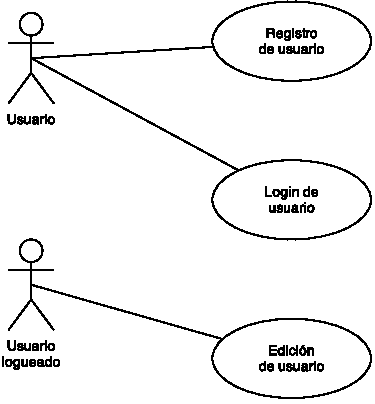
\includegraphics[width=0.5\textwidth]{4_analisis/diagrama_subsistema_gestion_usuarios}
  \caption{Casos de uso del subsistema de gestión de usuarios}
  \label{fig:subsistema-usuarios}
\end{figure}

\subsubsection{Caso de uso: registro de usuario}

\begin{description}
\item[Descripción] Un usuario no logueado se registra en la aplicación para poder dar de alta chequeos.
\item[Actores] \textit{Usuario}.
\item[Escenario principal] $\quad$
  \begin{enumerate}
  \item Un usuario decide registrarse en el sistema y accede al panel de registro.
  \item El \textit{usuario} introduce su nombre de usuario, dirección de correo electrónico y contraseña.
  \item El \textit{sistema} comprueba que los datos introducidos son correctos.
  \item El \textit{sistema} registra al usuario.
  \end{enumerate}
\item[Flujo alternativo] $\quad$
  \begin{description}
  \item[3a] Alguno de los datos introducidos es incompleto o no es correcto. El
    sistema informa al usuario del error.
  \item[3b] El nombre de usuario o dirección de correo electrónico ya han sido
    usados por otro usuario previamente. El sistema informa al usuario del error.
  \end{description}
\end{description}

\subsubsection{Caso de uso: login de usuario}


\begin{description}
\item[Descripción] Un usuario no logueado pero previamente registrado quiere hacer login en la aplicación.
\item[Actores] \textit{Usuario}.
\item[Escenario principal] $\quad$
  \begin{enumerate}
  \item Un usuario decide hacer login en el sistema.
  \item El \textit{usuario} accede al panel de login e introduce su nombre de usuario y contraseña.
  \item El \textit{sistema} comprueba que los datos introducidos son correctos.
  \item El \textit{sistema} loguea al usuario
  \end{enumerate}
\item[Flujo alternativo] $\quad$
  \begin{description}
  \item[3a] Alguno de los datos introducidos no tiene el formato correcto o está
    en blanco. El sistema informa al usuario del error.
  \item[3b] Los datos introducidos no corresponden a ningún usuario
    registrado. El sistema informa al usuario del error.
  \end{description}
\end{description}

\subsubsection{Caso de uso: edición de usuario}

\begin{description}
\item[Descripción] Un usuario logueado decide editar alguno de sus datos personales.
\item[Actores] \textit{Usuario logueado}.
\item[Escenario principal] $\quad$
  \begin{enumerate}
  \item El \textit{usuario} accede a su perfil de usuario a través del enlace \textit{Your profile}.
  \item El \textit{sistema} muestra los datos actuales.
  \item El \textit{usuario} edita los datos que quiera y envía el formulario.
  \item El \textit{sistema} comprueba los nuevos datos y guarda los cambios.
  \end{enumerate}
\item[Flujo alternativo] $\quad$
  \begin{description}
  \item[3a] Alguno de los nuevos datos no son válidos. El sistema informa del error al usuario.
  \end{description}
\end{description}

\subsection{Subsistema de gestión de grupos de chequeos}

Los casos de uso pertenecientes a este subsistema pueden verse en la figura~\ref{fig:subsistema-grupos}

\begin{figure}[hp]
  \centering
  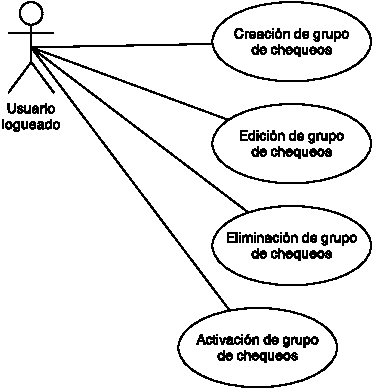
\includegraphics[width=0.5\textwidth]{4_analisis/diagrama_subsistema_gestion_grupos}
  \caption{Casos de uso del subsistema de gestión de grupos de chequeos}
  \label{fig:subsistema-grupos}
\end{figure}

\subsubsection{Caso de uso: creación de grupo de chequeos}

\begin{description}
\item[Descripción] Un usuario logueado decide crear un grupo de chequeos.
\item[Actores] \textit{Usuario logueado}.
\item[Escenario principal] $\quad$
  \begin{enumerate}
  \item El \textit{usuario} decide crear un nuevo grupo de chequeos.
  \item El \textit{usuario} pulsa en el botón de \textit{Añadir grupo}.
  \item El \textit{sistema} muestra el formulario para añadir nuevo grupo.
  \item El \textit{usuario} escribre el título del grupo.
  \item El \textit{sistema} valida el título introducido.
  \item El \textit{sistema} crea el nuevo grupo.
  \end{enumerate}
\item[Flujo alternativo] $\quad$

  \begin{description}
  \item[5a] El título introducido está en blanco o es inválido. El sistema
    informa al usuario del error.
  \end{description}
\end{description}


\subsubsection{Caso de uso: edición de grupo de chequeos}

\begin{description}
\item[Descripción] Un usuario logueado decide editar un grupo de chequeos.
\item[Actores] \textit{Usuario logueado}.
\item[Escenario principal] $\quad$
  \begin{enumerate}
  \item El \textit{usuario} decide editar un nuevo grupo de chequeos.
  \item El \textit{usuario} pulsa en el botón de \textit{Editar grupo} del grupo que quiera editar..
  \item El \textit{sistema} muestra el formulario para editar el grupo.
  \item El \textit{usuario} modifica el título del grupo.
  \item El \textit{sistema} valida el título introducido.
  \item El \textit{sistema} actualiza los datos del grupo.
  \end{enumerate}
\item[Flujo alternativo] $\quad$

  \begin{description}
  \item[5a] El título introducido está en blanco o es inválido. El sistema
    informa al usuario del error.
  \end{description}
\end{description}


\subsubsection{Caso de uso: eliminación de grupo de chequeos}

\begin{description}
\item[Descripción] Un usuario logueado decide eliminar un grupo de chequeos.
\item[Actores] \textit{Usuario logueado}.
\item[Escenario principal] $\quad$
  \begin{enumerate}
  \item El \textit{usuario} decide eliminar uno de sus grupos de chequeos.
  \item El \textit{usuario} pulsa en el botón de eliminar grupo.
  \item El \textit{sistema} muestra el formulario para confirmar la eliminación.
  \item El \textit{usuario} confirma la eliminación.
  \item El \textit{sistema} elimina los chequeos asociados al grupo.
  \item El \textit{sistema} elimina el grupo de chequeos.
  \end{enumerate}
\item[Flujo alternativo] $\quad$
  \begin{description}
  \item[3a] El \textit{usuario} no confirma la eliminación. El \textit{sistema}
    muestra la pantalla inicial.
  \end{description}
\end{description}

\subsubsection{Caso de uso: activación de grupo de chequeos}

\begin{description}
\item[Descripción] Un usuario logueado decide activar un grupo de chequeos.
\item[Actores] \textit{Usuario logueado}
\item[Escenario principal] $\quad$
  \begin{enumerate}
  \item El \textit{usuario} decide activar un grupo de chequeos.
  \item El \textit{usuario} pulsa en el botón de \textit{Activar grupo}.
  \item El \textit{sistema} itera por todos los chequeos pertenecientes al
    grupo, activando cada uno de ellos.
  \item El \textit{sistema} informa al usuario de que todos los chequeos han
    sido activados.
  \end{enumerate}

\item[Flujo alternativo] $\quad$
  \begin{description}
  \item[3a] El grupo no cuenta con chequeos. El \textit{sistema} no activa
    ningún chequeo.
  \end{description}
\end{description}

\subsection{Subsistema de gestión de chequeos}

Los casos pertenecientes a este subsistema pueden verse en la figura~\ref{fig:subsistema-chequeos}.

\begin{figure}[htbp]
  \centering
  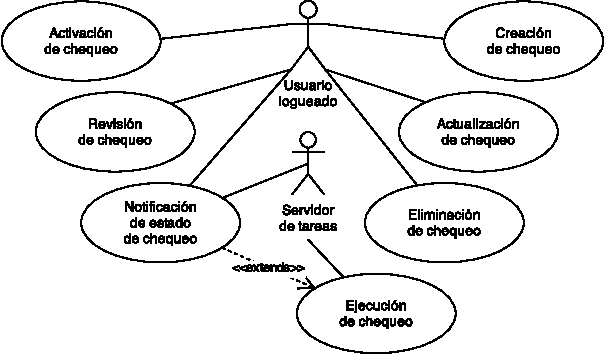
\includegraphics[width=0.7\textwidth]{4_analisis/diagrama_subsistema_gestion_chequeos}
  \caption{Casos de uso del subsistema de gestión de chequeos}
  \label{fig:subsistema-chequeos}
\end{figure}

\subsubsection{Caso de uso: creación de chequeo}

\begin{description}
\item[Descripción] Un usuario logueado decide crear un un chequeo dentro de un grupo.
\item[Actores] \textit{Usuario logueado}
\item[Escenario principal] $\quad$
  \begin{enumerate}
  \item El \textit{usuario} decide crear un chequeo dentro de un grupo de chequeos.
  \item El \textit{usuario} pulsa el botón de \textit{Añadir chequeo} de un grupo.
  \item El \textit{sistema} muestra el formulario de elección del tipo de chequeo.
  \item El \textit{usuario} elige el tipo de chequeo a añadir.
  \item El \textit{sistema} muestra el formulario con los campos según el tipo de chequeo elegido.
  \item El \textit{usuario} introduce los detalles del chequeo y envía el formulario.
  \item El \textit{sistema} recibe y comprueba que los datos son correctos.
  \item El \textit{sistema} da de alta el nuevo chequeo.
  \end{enumerate}
\item[Flujo alternativo] $\quad$
  \begin{description}
  \item[7a] Alguno de los datos introducidos no es correcto. El \textit{sistema}
    informa del error al usuario y muestra el formulario de nuevo.
  \end{description}
\end{description}


\subsubsection{Caso de uso: actualización de chequeo}

\begin{description}
\item[Descripción] Un usuario logueado decide editar un chequeo previamente creado..
\item[Actores] \textit{Usuario logueado}
\item[Escenario principal] $\quad$
  \begin{enumerate}
  \item El \textit{usuario} decide editar un chequeo dentro de un grupo de chequeos.
  \item El \textit{usuario} pulsa el botón de \textit{Editar chequeo}.
  \item El \textit{sistema} muestra el formulario con los campos rellenos con la información del chequeo elegido..
  \item El \textit{usuario} modifica los detalles del chequeo y envía el formulario.
  \item El \textit{sistema} recibe y comprueba que los datos son correctos.
  \item El \textit{sistema} actualiza el chequeo.
  \end{enumerate}
\item[Flujo alternativo] $\quad$
  \begin{description}
  \item[5a] Alguno de los datos introducidos no es correcto. El \textit{sistema}
    informa del error al usuario y muestra el formulario de nuevo.
  \end{description}
\end{description}

\subsubsection{Caso de uso: eliminación de chequeo}

\begin{description}
\item[Descripción] Un usuario logueado decide eliminar un chequeo previamente creado..
\item[Actores] \textit{Usuario logueado}
\item[Escenario principal] $\quad$
  \begin{enumerate}
  \item El \textit{usuario} decide eliminar un chequeo dentro de un grupo de chequeos.
  \item El \textit{usuario} pulsa el botón de \textit{Eliminar chequeo}.
  \item El \textit{sistema} muestra el formulario de confirmación de eliminación
  \item El \textit{usuario} confirma la eliminación del chequeo.
  \item El \textit{sistema} elimina el chequeo.
  \end{enumerate}
\item[Flujo alternativo] $\quad$
  \begin{description}
  \item[4a] El \textit{usuario} no confirma la eliminación del chequeo. El
    \textit{sistema} vuelve a la pantalla inicial.
  \end{description}
\end{description}

\subsubsection{Caso de uso: activación de chequeo}

\begin{description}
\item[Descripción] Un usuario logueado decide activar un chequeo.
\item[Actores] \textit{Usuario logueado}
\item[Escenario principal] $\quad$
  \begin{enumerate}
  \item El \textit{usuario} decide activar un chequeo dentro de un grupo de chequeos.
  \item El \textit{usuario} pulsa el botón de \textit{activar chequeo}.
  \item El \textit{sistema} activa el chequeo.
  \end{enumerate}
\end{description}

\subsubsection{Caso de uso: ejecución de chequeo}

\begin{description}
\item[Descripción] El servidor de tareas tiene que lanzar un chequeo periódico.
\item[Actores] \textit{Servidor de tareas}
\item[Escenario principal] $\quad$
  \begin{enumerate}
  \item El \textit{servidor de tareas} pide los chequeos activos.
  \item El \textit{sistema} devuelve los chequeos activos.
  \item El \textit{servidor de tareas} elige un chequeo activo.
  \item El \textit{servidor de tareas} ejecuta el chequeo.
  \item El \textit{sistema} devuelve el resultado del chequeo.
  \item El \textit{servidor de tareas} comprueba el resultado del chequeo,
    guardándolo en la base de datos y, si difere del estado anterior del
    chequeo, lanzando el \textit{Caso de uso: notificación de estado de chequeo}.
  \end{enumerate}
\item[Flujo alternativo] $\quad$
  \begin{description}
  \item[2a] No hay chequeos activos. El \textit{sistema} devuelve una lista
    vacía. El \textit{servidor de tareas} permanece en reposo.
  \end{description}
\end{description}

\subsubsection{Caso de uso: noitificación de estado de chequeo}

\begin{description}
\item[Descripción] El servidor de tareas detecta un cambio de estado y lanza notificación.
\item[Actores] \textit{Servidor de tareas}
\item[Escenario principal] $\quad$
  \begin{enumerate}
  \item El \textit{servidor de tareas} detecta un cambio de estado de un chequeo.
  \item El \textit{servidor de tareas} comprueba el campo
    \textit{Notificar\_correo} del chequeo.
  \item El \textit{servidor de tareas} lanza una notificación por correo electrónico.
  \item El \textit{sistema} envía la notificación al usuario dueño del chequeo.

  \item El \textit{servidor de tareas} comprueba el campo
    \textit{Notificar\_android} del chequeo.
  \item El \textit{servidor de tareas} lanza una notificación Android.
  \item El \textit{sistema} envía la notificación al usuario dueño del chequeo.

  \end{enumerate}
\item[Flujo alternativo] $\quad$
  \begin{description}
  \item[2a] El chequeo no tiene activa la opción \textit{Notificar\_correo}. El
    \textit{servidor de tareas} no envía la notificación por correo.
  \item[5a] El chequeo no tiene activa la opción \textit{Notificar\_android}. El
    \textit{servidor de tareas} no envía la notificación por Android.
  \item[5b] El usuario no tiene dispositivo Android dado de alta. El
    \textit{servidor de tareas} no envía la notificación por Android.
  \end{description}
\end{description}

\section{Modelo de comportamiento}

Basándonos en los casos de uso anteriores se crea el modelo de comportamiento,
compuesto de diagramas de secuencia, en los que se identificarán las operaciones
del sistema, y de lo contratos de estas operaciones.

\section{Modelo de interfaz de usuario}

\subsection{Modelo de navegación}

El modelo de navegación de la aplicación web se presenta en la
figura~\ref{fig:modelo-navegacion-web}. El modelo de navegación de la aplicación
Android se presenta en la figura~\ref{fig:modelo-navegacion-android}

\begin{figure}[H]
  \centering
  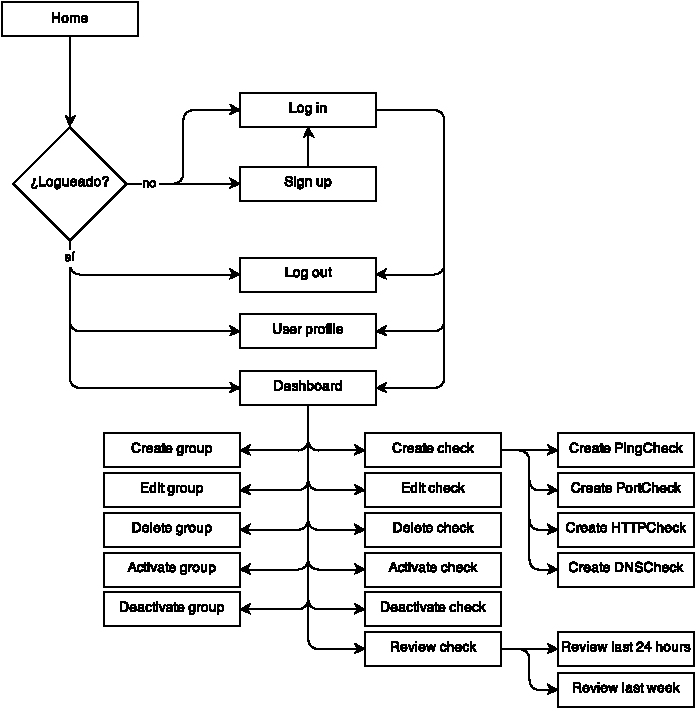
\includegraphics[width=0.8\textwidth]{4_analisis/diagrama_navegacion}
  \caption{Modelo de navegación de la aplicación web}
  \label{fig:modelo-navegacion-web}
\end{figure}

\begin{figure}[H]
  \centering
  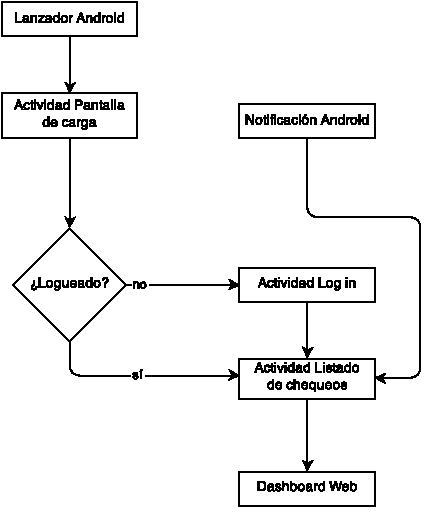
\includegraphics[width=0.6\textwidth]{4_analisis/diagrama_navegacion_android}
  \caption{Modelo de navegación de la aplicación Android}
  \label{fig:modelo-navegacion-android}
\end{figure}

% \section{Especificación de requisitos del sistema}

% \subsection{Requisitos de interfaces externas}
% En esta sección describiremos los requisitos que deben cumplir las interfaces
% con el hardware, el software y el usuario.

% En cuanto a la comunicación con el subsistema gráfico y de E/S, utilizaremos la
% biblioteca Gosu~\cite{gosu}, un proyecto de software libre que proporciona un
% framework de desarrollo de videojuegos 2D, multiplataforma y muy sencillo de
% usar. Para el acceso al subsistema de audio, tal y como se ha comentado en la
% sección anterior, optamos por utilizar la API simple de PulseAudio.

% \textbf{oFlute} dispondrá de una resolución fija de 800 por 600 píxeles,
% requisito fácilmente alcanzable en cualquier ordenador actual. Al tratar con un
% público objetivo joven, los gráficos y la interactividad deberán ser sencillos y
% fáciles de interpretar. Así, se ha trabajado en limitar la interacción del
% usuario con la aplicación al uso del ratón y, obviamente, del instrumento
% musical, en este caso la flauta dulce. La navegación resultante de este
% planteamiento queda reflejada en el siguiente diagrama:

% \begin{figure}[h!]
%   \centering
%   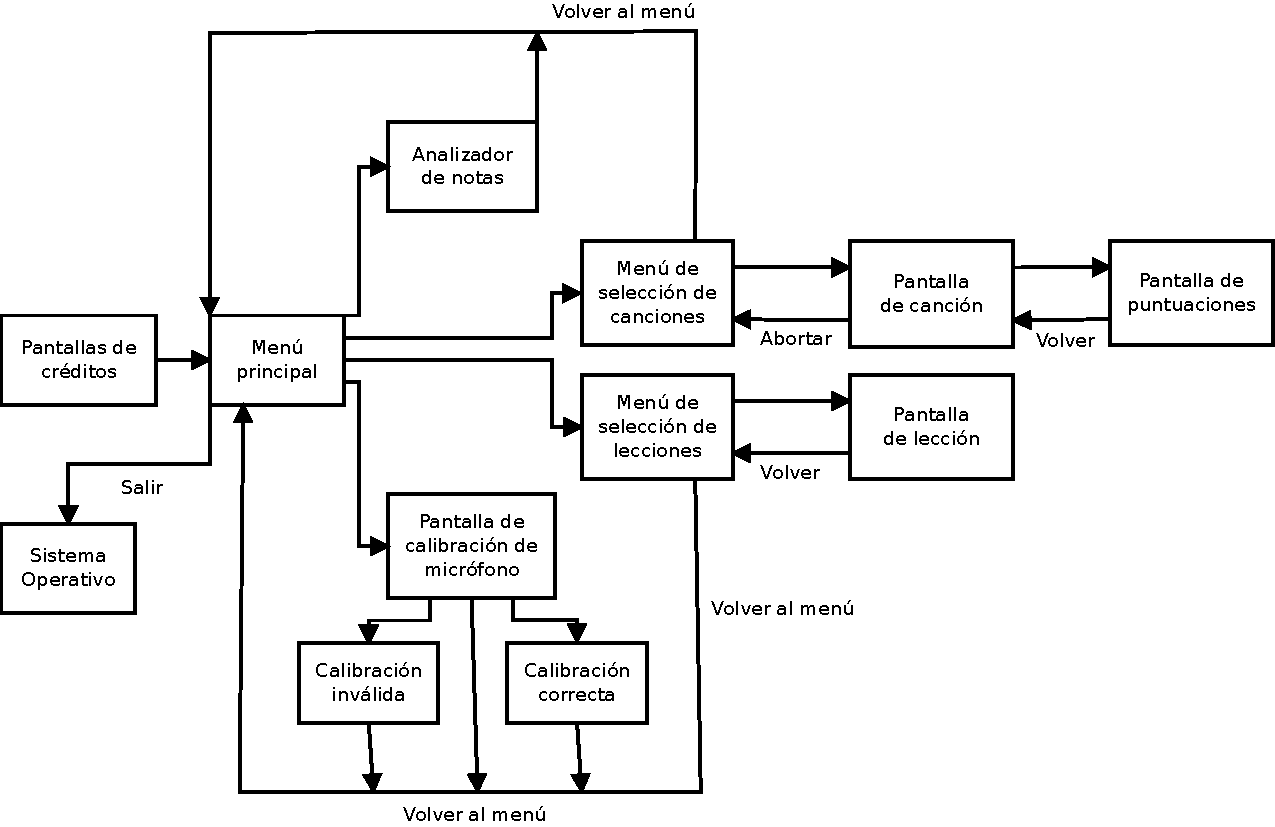
\includegraphics[width=0.9\textwidth]{4_analisis/imagen_diagrama_de_flujo}
%   \caption{Diagrama de flujo de las pantallas de oFlute}
% \end{figure}

% \pagebreak

% Inicialmente, deberán aparecer unas pantallas de crédito con información sobre
% el desarrollador y sobre el propio videojuego. Tras las mismas, que deberá ser
% posible omitir, habrá de aparecer el \textbf{menú principal}, con las cinco
% opciones posibles.

% \begin{figure}[h!]
%   \centering
%   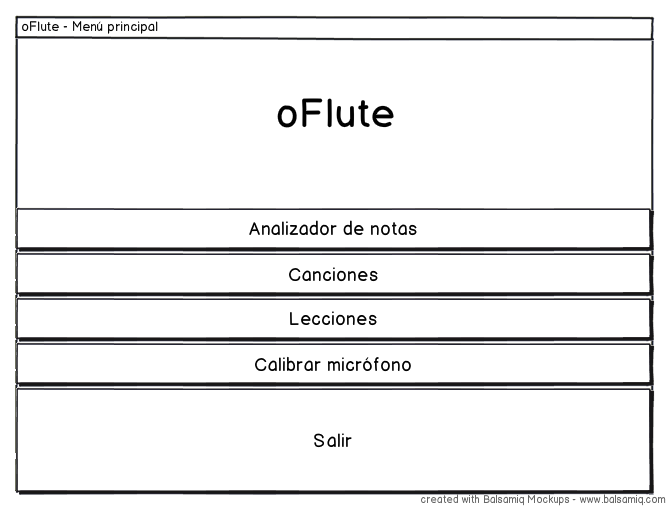
\includegraphics[width=0.6\textwidth]{4_analisis/imagen_mockup_menu_principal}
%   \caption{Maqueta del menú principal}
% \end{figure}

% \pagebreak

% Las opciones que se incluirán son:
% \begin{itemize}
% \item \textbf{Analizador de notas}: comprobar las notas que tocamos sobre un
%   pentagrama.
% \item \textbf{Canciones}: sección principal del juego, en el que aparecerán las
%   canciones a tocar.
% \item \textbf{Lecciones}: sección de lecciones de aprendizaje.
% \item \textbf{Calibrar micrófono}, para ajustarse al nivel de ruido ambiental.
% \item \textbf{Salir} al sistema operativo.
% \end{itemize}

% La siguiente pantalla a modelar será el \textbf{analizador de
%   notas}. Simplemente mostrará el logotipo del videojuego a un lado, y un
% pentagrama al otro, que se actualizará con la nota detectada por el
% micrófono. También contendrá un botón \textit{volver} para ir al menú principal.

% \begin{figure}[h!]
%   \centering
%   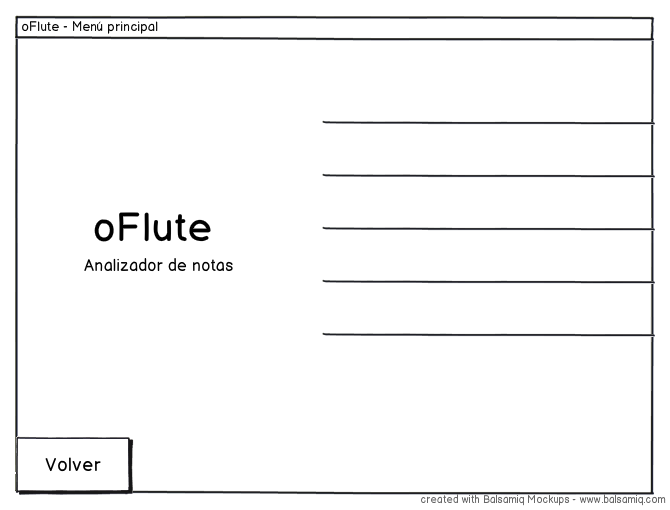
\includegraphics[width=0.6\textwidth]{4_analisis/imagen_mockup_analizador}
%   \caption{Maqueta de la sección \textit{analizador de notas}}
% \end{figure}

% La segunda sección a la que se podrá ir desde el menú principal será la de
% \textbf{canciones}. Inicialmente, la primera pantalla será la de
% \textbf{selección de canción}, que contendrá el logotipo del juego, un botón
% para volver al menú principal, y un menú dinámico de canciones que nos permitirá
% elegir el tema a interpretar.

% \begin{figure}[h!]
%   \centering
%   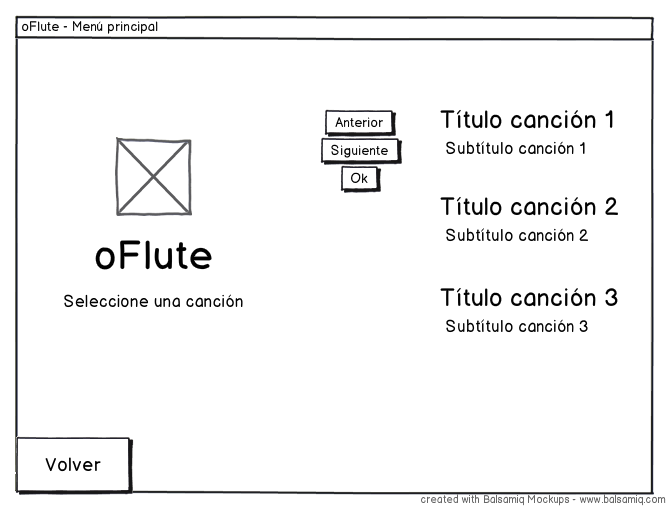
\includegraphics[width=0.6\textwidth]{4_analisis/imagen_mockup_seleccionar_cancion}
%   \caption{Maqueta del menú de selección de canción}
% \end{figure}

% Una vez seleccionada la canción, pasaremos a la zona de \textbf{interpretación
%   de canción}. Contendrá un pentagrama que ocupará todo el ancho de la pantalla,
% con una línea que indicará la zona donde empezar a tocar las notas que
% aparezcan. Además, en la parte superior habrá un indicador con la puntuación
% obtenida y, abajo, una barra de progreso que nos indicará cuánto queda de
% canción.

% \begin{figure}[h!]
%   \centering
%   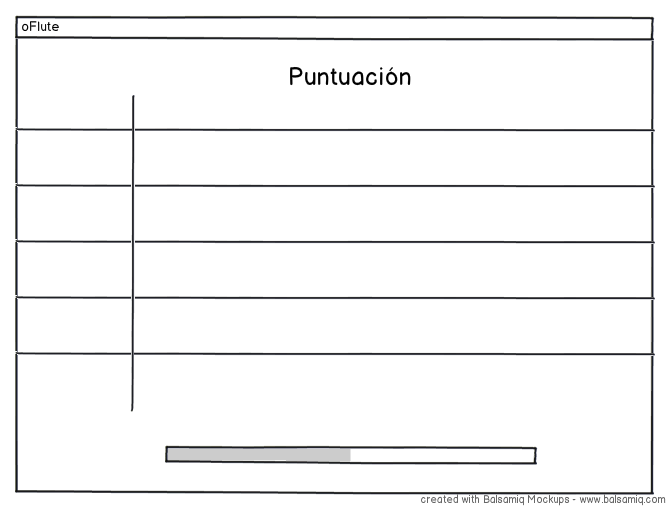
\includegraphics[width=0.6\textwidth]{4_analisis/imagen_mockup_reproducir_cancion}
%   \caption{Maqueta de la pantalla de interpretación de canción}
% \end{figure}

% \pagebreak

% Al completar la interpretación de la canción, aparecerá la \textbf{sección de
%   resultados}. Contendrá el logotipo del juego, el título y subtítulo de la
% canción, y un cuadro con información sobre nuestra interpretación, representada
% en forma de porcentaje de aciertos. Además, en la zona inferior aparecerá un
% mensaje de ánimo dependiendo del resultado obtenido.

% \begin{figure}[h!]
%   \centering
%   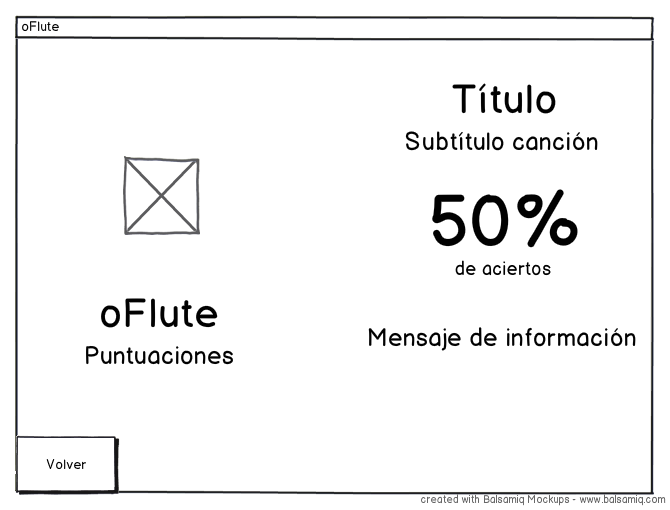
\includegraphics[width=0.6\textwidth]{4_analisis/imagen_mockup_puntuaciones}
%   \caption{Maqueta de la pantalla de puntuaciones}
% \end{figure}

% La pantalla de \textbf{selección de lecciones}, a la que se llega desde el menú
% principal, contendrá el título, una imagen decorativa, y varios botones para
% navegar entre las lecciones cargadas en el sistema. Se mostrará el título y la
% descripción de cada lección, así como un botón para comenzar.

% \begin{figure}[h!]
%   \centering
%   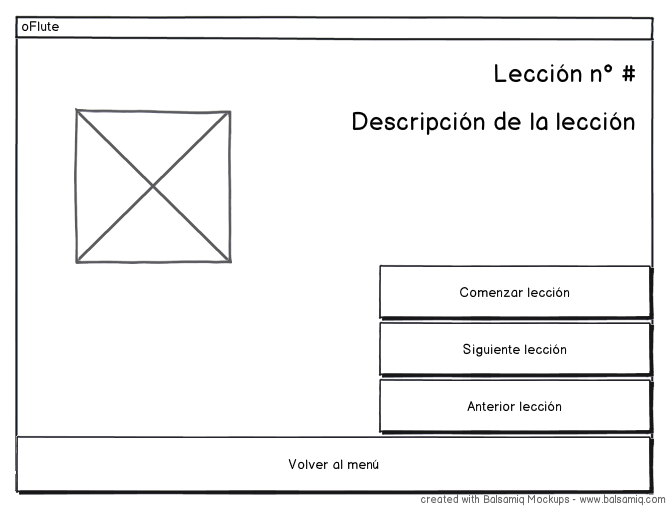
\includegraphics[width=0.6\textwidth]{4_analisis/imagen_mockup_seleccionar_leccion}
%   \caption{Maqueta del menú de selección de lecciones}
% \end{figure}

% Una vez elegida una lección, pasaremos a la pantalla de reproducción de
% lecciones. Dada la naturaleza \textbf{dinámica} de esta sección, cada lección
% podrá tener una apariencia y elementos distintos. El único elemento común entre
% todas las lecciones será el botón de \textbf{volver al menú}.

% \subsection{Requisitos funcionales}

% \textbf{oFlute} se basa en los siguientes requisitos funcionales:
% \begin{itemize}
% \item Poder terminar la aplicación pulsando el botón de cierre en cualquier
%   instante.
% \item Comprobar la correcta interpretación de notas individuales mediante el
%   analizador de notas.
% \item Calibrar el micrófono de forma que el sistema se pueda adaptar al ruido
%   ambiental del entorno.
% \item Navegar por toda la aplicación de forma sencilla utilizando solo el ratón.
% \item Elegir entre varias canciones a interpretar, cada una con su título y
%   subtítulo informativos.
% \item Interpretar las canciones mediante el uso de la flauta, siguiendo el
%   pentagrama en pantalla.
% \item Elegir entre bastantes lecciones informativas, poder ejecutarlas y
%   seguirlas.
% \item Capacidad de añadir nuevas lecciones y canciones de forma sencilla.
% \end{itemize}

% \subsection{Requisitos de rendimiento}

% La aplicación \textbf{oFlute} precisa de unos requisitos bastante básicos,
% que en su mayor parte se reducen a cuatro puntos principales:
% \begin{itemize}
% \item Posesión de una tarjeta de sonido o subsistema de audio similar con un
%   micrófono, para poder captar el sonido de la flauta.
% \item Pantalla con una resolución de, al menos, 800 por 600 píxeles.
% \item Sistema gráfico compatible con OpenGL.
% \item Dispositivo apuntador, como un ratón.
% \end{itemize}

% La práctica totalidad de los ordenadores personales de la actualidad cumplen los
% citados requisitos.

% \subsection{Requisitos del sistema software}
% El sistema de software deberá cumpliar los requisitos siguientes:
% \begin{itemize}
% \item Deberá funcionar en cualquier sistema \textbf{GNU/Linux} con los
%   requisitos anteriormente indicados.
% \item Deberá limitarse el número de dependencias, así como facilitar al máximo
%   la instalación de las que resultasen imprescindibles.
% \item El uso del teclado quedará en segundo plano, haciendo posible utilizar la
%   aplicación completamente con el ratón.
% \item Al tratarse de un público objetivo juvenil, la aplicación deberá ser
%   dinámica, intuitiva y fácil de usar, y la apariencia debe ser agradable.
% \item Se evitará el uso de constantes y recursos dentro del código de la
%   aplicación, utilizando como alternativa ficheros para representar las
%   lecciones y las canciones.
% \end{itemize}

% \section{Modelo de casos de uso}

% A la hora de modelar los casos de uso del sistema, hemos optado por utilizar
% notación \textit{UML}, siguiendo los siguientes pasos:
% \begin{itemize}
% \item Identificación de los usuarios del sistema y sus roles.
% \item Para cada rol, determinar las formas de interactuar con el sistema.
% \item Creación de casos de uso para los objetivos que debe cumplir la aplicación.
% \item Modularización de los casos de usos mediante la implementación de
%   relaciones de inclusión o extensión.
% \end{itemize}

% \subsection{Diagrama de casos de uso}

% \begin{figure}[h!]
%   \centering
%   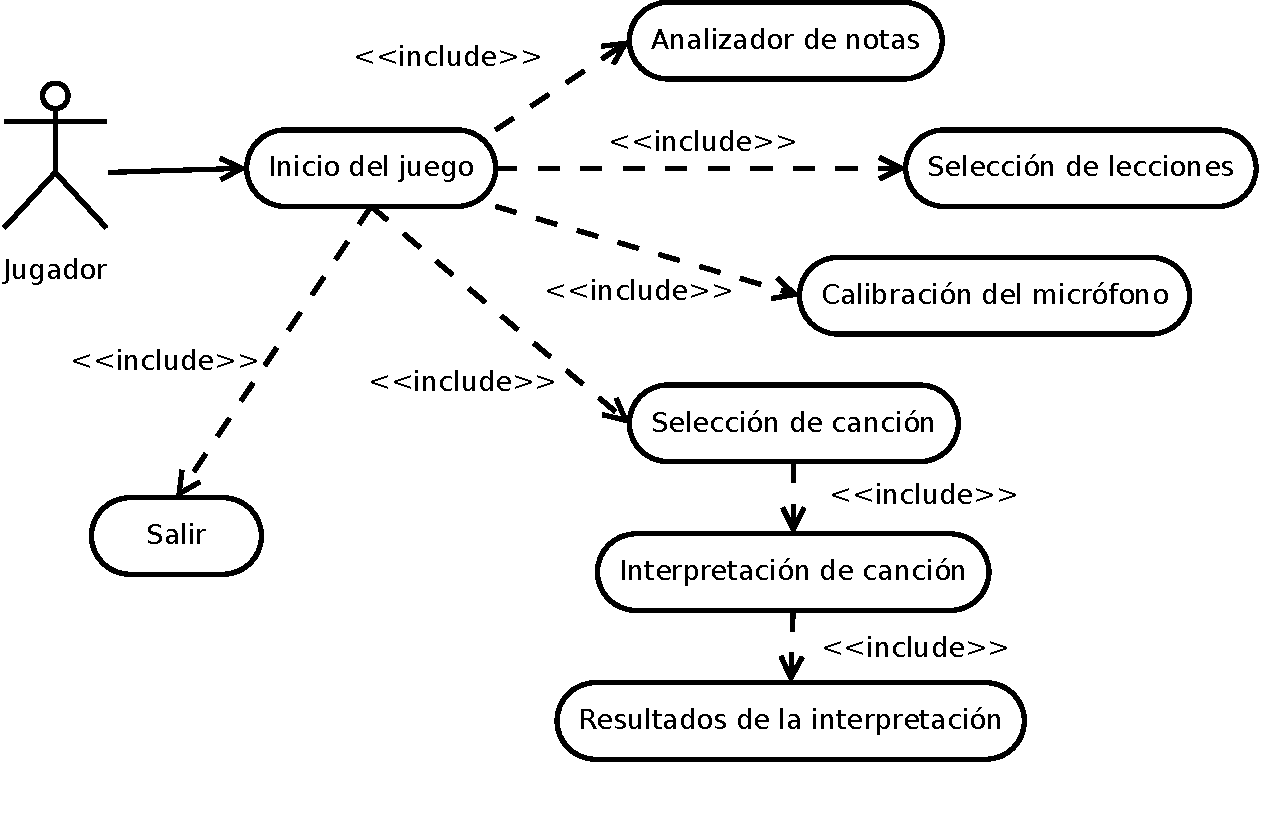
\includegraphics[width=0.81\textwidth]{4_analisis/imagen_diagrama_de_casos_de_uso}
%   \caption{Diagrama de casos de uso}
% \end{figure}


% \subsection{Descripción de los casos de uso}

% \subsubsection{Caso de uso: inicio del juego}
% \begin{description}
% \item [Descripción] Se muestran los créditos del juego, la pantalla de
%   presentación, y finalmente el menú principal, desde donde se accederá al
%   resto de secciones del juego.
% \item [Actores] \jugador.
% \item [Precondiciones] Ninguna.
% \item [Postcondiciones] Ninguna.
% \item [Escenario principal] $\quad$
%   \begin{enumerate}
%   \item El \jugador\ inicia la aplicación.
%   \item El \sistema\ inicializa el subsistema gráfico.
%   \item El \sistema\ muestra la pantalla de créditos y la pantalla de
%     presentación de la aplicación.
%   \item El \sistema\ muestra el menú principal en la pantalla.
%   \item El \jugador\ selecciona la opción \textit{Canciones}.
%   \item El \sistema\ accede a la pantalla de \textit{Selección de canción}.
%   \end{enumerate}
% \item[Extensiones --- flujo alternativo] $\quad$
%   \begin{description}
%   \item [*a] El \jugador\ cierra la ventana.
%     \begin{enumerate}
%     \item El \sistema\ libera los recursos y sale de la aplicación.
%     \end{enumerate}
%   \item [4a] El \jugador\ selecciona la opción \textit{Analizador de Notas}.
%     \begin{enumerate}
%     \item El \sistema\ accede a la pantalla del analizador de notas.
%     \end{enumerate}

%   \item[4b] El \jugador\ selecciona la opción \textit{Lecciones}.
%     \begin{enumerate}
%     \item El \sistema\ accede a la pantalla de \textit{Selección de lecciones}.
%     \end{enumerate}
%   \item[4c] El \jugador\ selecciona la opción \textit{Calibrar micrófono}.
%     \begin{enumerate}
%     \item El \sistema\ accede a la pantalla de calibración de micrófono.
%     \end{enumerate}
%   \item [4d] El \jugador\ selecciona la opción Salir.
%     \begin{enumerate}
%     \item El \sistema\ libera los recursos y sale de la aplicación.\\
%     \end{enumerate}
%   \end{description}  
% \end{description}


% \subsubsection{Caso de uso: selección de canción}

% \begin{description}
% \item [Descripción] Al \jugador\ se le muestra una lista de las canciones
%   detectadas, y éste debe elegir entre ellas la que desea interpretar, o volver
%   al menú princial.
% \item [Actores] \jugador.
% \item [Precondiciones] Ninguna.
% \item [Postcondiciones] Una canción queda seleccionada.
% \item [Escenario principal] $\quad$
%   \begin{enumerate}
%   \item El \jugador\ accede, desde el menú principal, al panel de selección de canciones.
%   \item El \sistema\ busca las canciones dadas de alta en el juego y muestra un menú con las mismas.
%   \item El \jugador\ navega entre las canciones listadas y selecciona una de ellas, pulsando finalmente el botón \textit{Ok}.
%   \item El \sistema\ carga la canción y pasa a la pantalla de interpretación de canciones.
%   \end{enumerate}
% \item[Extensiones --- flujo alternativo] $\quad$
%   \begin{description}
%   \item [*a] El \jugador\ cierra la ventana.
%     \begin{enumerate}
%     \item El \sistema\ libera los recursos y sale de la aplicación.
%     \end{enumerate}
%   \item [3a] El \jugador\ selecciona la opción \textit{Volver}.
%     \begin{enumerate}
%     \item El \sistema\ muestra la animación de cierre y vuelve al menú principal.
%     \end{enumerate}
%   \end{description}  
% \end{description}


% \subsubsection{Caso de uso: interpretación de canción}

% \begin{description}
% \item [Descripción] Tras haber elegido la canción a interpretar, se muestra una
%   partitura con las notas que el \jugador\ deberá tocar para conseguir la puntuación deseada.
% \item [Actores] \jugador.
% \item [Precondiciones] Se ha elegido una canción.
% \item [Postcondiciones] Se completa la interpretación de la canción, obteniendo una calificación
% \item [Escenario principal] $\quad$
%   \begin{enumerate}
%   \item El \sistema\ carga la canción, leyendo las notas, y muestra en pantalla,
%     mediante animaciones, el marcador de puntos y el pentagrama.
%   \item El \sistema\ comienza a mostrar notas en el pentagrama, que van
%     deslizándose hacia el lado izquierdo, en el que se encuentra la aguja de
%     reproducción, e inicia el análisis del sonido.
%   \item El \jugador\, al llegar la nota a la aguja de reproducción, toca la
%     flauta con la altura y la duración correcta, de forma que el micrófono sea
%     capaz de captar el sonido.
%   \item El \sistema\ analiza el sonido que captura el micrófono y detecta la nota que toca el usuario.
%   \item El \sistema\ determina que la nota es la correcta y suma los puntos correspondientes.
%   \item Mientras existan más notas, se vuelve al punto 2.
%   \item El \sistema\ determina que no hay más notas que mostrar, e inicia las
%     animaciones para ocultar los elementos en pantalla.
%   \item El \sistema\ pasa a la sección de \textit{Resultados de la interpretación}.
%   \end{enumerate}
% \item[Extensiones --- flujo alternativo] $\quad$
%   \begin{description}

%   \item [*a] El \jugador\ cierra la ventana.
%     \begin{enumerate}
%     \item El \sistema\ libera los recursos y sale de la aplicación.
%     \end{enumerate}

%   \item[*b] El \jugador\ pulsa la tecla \texttt{escape}.
%     \begin{enumerate}
%     \item El \sistema\ vuelve a la pantalla de \textit{selección de canción}.
%     \end{enumerate}

%   \item [3a] El \jugador\ toca el instrumento con intensidad insuficiente o nula
%     y el sonido no llega al sistema.
%     \begin{enumerate}
%     \item El \sistema\ representa esta inconsistencia como un silencio.
%     \end{enumerate}

%   \item [4a] El \sistema\ no es capaz de determinar fehacientemente la nota que
%     toca el usuario.
%     \begin{enumerate}
%     \item El \sistema\ representa esta inconsistencia como un silencio.
%     \end{enumerate}

%   \item[5a] El \sistema\ determina que la nota tocada por el usuario no es la
%     que corresponde a la partitura.
%     \begin{enumerate}
%     \item El \sistema\ ignora esta situación y no suma los puntos al marcador.
%     \end{enumerate}

%   \end{description}  
% \end{description}

% \subsubsection{Caso de uso: resultados de la interpretación}

% \begin{description}
% \item [Descripción] Después de interpretar las notas de la partitura, se
%   muestran los datos obtenidos del análisis de las notas tocadas por el \jugador.
% \item [Actores] \jugador.
% \item [Precondiciones] Se ha elegido e interpretado una canción.
% \item [Postcondiciones] Se completa la partida actual.
% \item [Escenario principal] $\quad$
%   \begin{enumerate}
%   \item El \sistema\ compara la puntuación conseguida con la máxima puntuación
%     obtenible, y genera un porcentaje de aciertos.
%   \item El \sistema\ muestra, mediante animaciones, un mensaje con información
%     sobre la canción y sobre la interpretación del \jugador\, representada
%     mediante un porcentaje de aciertos.
%   \item El \sistema\ muestra un mensaje variable en función del número de
%     aciertos conseguido.
%   \item El \jugador\ revisa su puntuación y pulsa el botón \textit{volver} para
%     ir de vuelta al menú de \textit{selección de canción}.
%   \end{enumerate}
% \item[Extensiones --- flujo alternativo] $\quad$
%   \begin{description}

%   \item [*a] El \jugador\ cierra la ventana.
%     \begin{enumerate}
%     \item El \sistema\ libera los recursos y sale de la aplicación.
%     \end{enumerate}

%   \item[4a] El \jugador\ pulsa la tecla \texttt{escape}.
%     \begin{enumerate}
%     \item El \sistema\ vuelve a la pantalla de \textit{selección de canción}.
%     \end{enumerate}

%   \end{description}  
% \end{description}


% \subsubsection{Caso de uso: analizador de notas}

% \begin{description}
% \item [Descripción] El \jugador\ elige la opción \textit{analizador de notas} en
%   el menú principal y es llevado a esta sección, en la que el sistema
%   representará gráficamente la nota que esté tocando con la flauta en cada
%   instante, sin otra interacción
% \item [Actores] \jugador.
% \item [Precondiciones] Ninguna.
% \item [Postcondiciones] Ninguna
% \item [Escenario principal] $\quad$
%   \begin{enumerate}
%   \item El \jugador\ accede, desde el menú principal, al panel del analizador de notas.
%   \item El \sistema\ muestra, mediante animaciones, la pantalla de la sección,
%     representada mediante una fracción de partitura en la que se representará la
%     nota que esté tocando el \jugador\ en cada momento.
%   \item El \sistema\ inicia el análisis del sonido.
%   \item El \jugador\ toca la nota que desee con su flauta, de forma que el
%     micrófono sea capaz de captar el sonido.
%   \item El \sistema\ analiza el sonido que captura el micrófono y detecta la
%     nota que toca el usuario.
%   \item El \sistema\ muestra en pantalla la nota, sobre la partitura,
%     correspondiente a lo que ha tocado el usuario.
%   \item Se repite el flujo desde el punto 4, mientras el \jugador\ no pulse en
%     el botón volver.
%   \item El \jugador\ pulsa en el botón \textit{volver}.
%   \item El \sistema\ inicia las animaciones para ocultar los elementos en pantalla.
%   \item El \sistema\ vuelve al menú principal.
%   \end{enumerate}
% \item[Extensiones --- flujo alternativo] $\quad$
%   \begin{description}

%   \item [*a] El \jugador\ cierra la ventana.
%     \begin{enumerate}
%     \item El \sistema\ libera los recursos y sale de la aplicación.
%     \end{enumerate}

%   \item[*b] El \jugador\ pulsa la tecla \texttt{escape}.
%     \begin{enumerate}
%     \item El \sistema\ vuelve al menú principal.
%     \end{enumerate}

%   \item [4a] El \jugador\ toca el instrumento con intensidad insuficiente o nula
%     y el sonido no llega al sistema.
%     \begin{enumerate}
%     \item El \sistema\ representa esta inconsistencia como un silencio.
%     \end{enumerate}

%   \item [5a] El \sistema\ no es capaz de determinar fehacientemente la nota que
%     toca el usuario.
%     \begin{enumerate}
%     \item El \sistema\ representa esta inconsistencia como un silencio.
%     \end{enumerate}
%   \end{description}  
% \end{description}

% \subsubsection{Caso de uso: calibración de micrófono}
% \begin{description}
% \item [Descripción] El \jugador\ elige la opción \textit{calibrar micrófono} en
%   el menú principal y es llevado a esta sección, en la que el \sistema\ calibrará
%   el micrófono de forma que sea posible aislar el sonido de la flauta del ruido
%   ambiental.
% \item [Actores] \jugador.
% \item [Precondiciones] Ninguna.
% \item [Postcondiciones] El \sistema\ obtiene un valor umbral con el que
%   discernir entre el sonido del instrumento y el ruido ambiente.
% \item [Escenario principal] $\quad$
%   \begin{enumerate}
%   \item El \jugador\ accede, desde el menú principal, al panel de calibración del micrófono.
%   \item El \sistema\ muestra la sección, indicando con un mensaje que el usuario
%     debe pulsar la tecla \texttt{escape} para iniciar la calibración.
%   \item El \jugador\ pulsa la tecla \texttt{escape} y se mantiene en silencio.
%   \item El \sistema\ inicia el análisis del sonido, guardando durante dos
%     segundos los valores de ruido que lee del micrófono.
%   \item El \sistema\ calcula, a partir de los valores leídos, el umbral de
%     ruido, y muestra un mensaje informando del final del proceso.
%   \item El \jugador\ pulsa la tecla \texttt{escape} y el \sistema\ vuelve al
%     menú principal.
%   \end{enumerate}
% \item[Extensiones --- flujo alternativo] $\quad$
%   \begin{description}

%   \item [*a] El \jugador\ cierra la ventana.
%     \begin{enumerate}
%     \item El \sistema\ libera los recursos y sale de la aplicación.
%     \end{enumerate}

%   \item[*b] El \jugador\ pulsa la tecla \texttt{escape}.
%     \begin{enumerate}
%     \item El \sistema\ cancela la calibración y vuelve al menú principal.
%     \end{enumerate}

%   \item [5a] El \sistema\ encuentra valores inválidos al leer el ruido
%     ambiental.
%     \begin{enumerate}
%     \item El \sistema\ informa al usuario del fallo del proceso de calibración.
%     \item El \jugador\ pulsa la tecla \texttt{escape} y el \sistema\ vuelve al
%       menú principal.
%     \end{enumerate}
%   \end{description}  
% \end{description}

% \subsubsection{Caso de uso: selección de lecciones}
% \begin{description}
% \item [Descripción] El \jugador\ elige la opción \textit{lecciones} en el menú
%   principal y es llevado a esta sección, en la que el \sistema\ mostrará una
%   lista de lecciones cargadas, entre las que el usuario deberá elegir.
% \item [Actores] \jugador.
% \item [Precondiciones] Ninguna.
% \item [Postcondiciones] Se ha elegido una lección
% \item [Escenario principal] $\quad$
%   \begin{enumerate}
%   \item El \jugador\ accede, desde el menú principal, al panel de selección de lecciones.
%   \item El \sistema\ carga la lista de secciones y muestra, mediante
%     animaciones, el panel, preseleccionando por defecto la primera lección.
%   \item El \jugador\ utiliza los botones de la sección para elegir una de las
%     lecciones, y activarla pulsando \textit{comenzar lección}.
%   \item El \sistema\ oculta de forma animada el panel de selección de lecciones.
%   \item El \sistema\ lee el fichero \texttt{xml} asociado a la lección indicada,
%     cargando los elementos que la componen y las animaciones que se ejecutarán.
%   \item El \sistema\ ejecuta las animaciones correspondientes a los elementos
%     multimedia de la lección.
%   \end{enumerate}
% \item[Extensiones --- flujo alternativo] $\quad$
%   \begin{description}

%   \item [*a] El \jugador\ cierra la ventana.
%     \begin{enumerate}
%     \item El \sistema\ libera los recursos y sale de la aplicación.
%     \end{enumerate}

%   \item[2a] El \sistema\ detecta que una de las lecciones leídas no está
%     correctamente construída.
%     \begin{enumerate}
%     \item El \sistema\ informa del error en el \textit{log} del programa y omite
%       la carga de esa lección.
%     \end{enumerate}

%   \item[3a] El \jugador\ pulsa la tecla \texttt{escape}.
%     \begin{enumerate}
%     \item El \sistema\ vuelve al menú principal.
%     \end{enumerate}

%   \item[6a] El \jugador\ pulsa la tecla \texttt{escape}.
%     \begin{enumerate}
%     \item El \sistema\ vuelve al menú de selección de lecciones.
%     \end{enumerate}

%   \end{description}  
% \end{description}

% \section{Modelo conceptual de datos}

% El modelo conceptual de datos representa, de forma esquemática, las clases que
% modelan el sistema y las relaciones que existen entre ellas, además de una
% pequeña introducción a su utilidad. 

% \begin{description}
% \item[Juego] Clase de control general. Gestiona el flujo de ejecución principal,
%   así como de la gestión de estados, que permite pasar de una sección a otra del
%   juego.
% \item[Estado] Clase base para los diferentes estados del juego. Las clases
%   correspondientes a las secciones se basarán en esta clase para interactuar con
%   el gestor de estados y poder pasar de una parte del juego a otra.
% \item[EstadoMenú] Representa el estado de juego para el menú principal, desde el
%   que se accede al resto de opciones del juego. 
% \item[EstadoAnalizador] Representa el estado del analizador básico de
%   notas. Contendrá los elementos necesarios para iniciar el análisis del audio,
%   así como los elementos de la interfaz.
% \item[EstadoCalibrarMicro] Representa el estado en el que se calibra el
%   micrófono. Al igual que la clase \textit{EstadoAnalizador}, deberá ser capaz
%   de acceder al sistema de audio para poder leer el volumen ambiente y así
%   calibrar el micrófono.
% \item[EstadoImagenFija] Modela una imagen fija a modo de pantalla de créditos,
%   de forma que sea sencillo añadir imágenes al inicio del juego, como firmas de
%   desarrolladores, logotipos de patrocinadores, etcétera.
% \item[EstadoMenúCanciones] Comprende el menú de selección de canciones, que se
%   encargará de leer los ficheros de canciones disponibles. Además, también se
%   encargará de lanzar las canciones en forma de estados secundarios.
% \item[EstadoCanción] Corresponde a la canción que se va a interpretar, lanzada desde
%   el estado \textit{EstadoMenuCanciones}.
% \item[EstadoMenúLecciones] Corresponde al menú de elección de lecciones, que
%   leerá y listará los ficheros de lección disponibles, y se encargará de lanzar
%   la lección elegida.
% \item[EstadoLección] Corresponde a la canción elegida desde el menú
%   \textit{EstadoMenúLecciones}.
% \item[Analizador] Controla la gestión del subsistema de audio y el análisis de
%   la entrada. Deberá proporcionar información sobre el volumen de la entrada
%   (para la calibración del micrófono) así como de la nota detectada en cada
%   instante.
% \item[Animación] Se encargará de facilitar la creación de animaciones en forma
%   de interpolación de valores, válidas para cambios de posición, opacidad,
%   etcétera.
% \item[Elemento] Esta clase de ayuda facilitará la carga y dibujado de elementos
%   para la interfaz, además de servir de capa de abstracción para las
%   animaciones.
% \item[ElementoImagen] Especialización de la clase \textit{Elemento} para
%   imágenes.
% \item[ElementoTexto] Especialización de la clase \textit{Elemento} para textos.
% \item[ElementoCombinado] Especialización de la clase \textit{Elemento} que
%   combina imagen y texto, a usar en casos como los botones del menú.
% \item[SistemaPartículas] Representa un sistema de partículas simple, para
%   generar efectos de destellos y fuegos artificiales.
% \item[Nota] Simboliza cada una de las notas cargadas que componen una canción.
% \end{description}

% \begin{figure}[htp!]
%   \centering
%   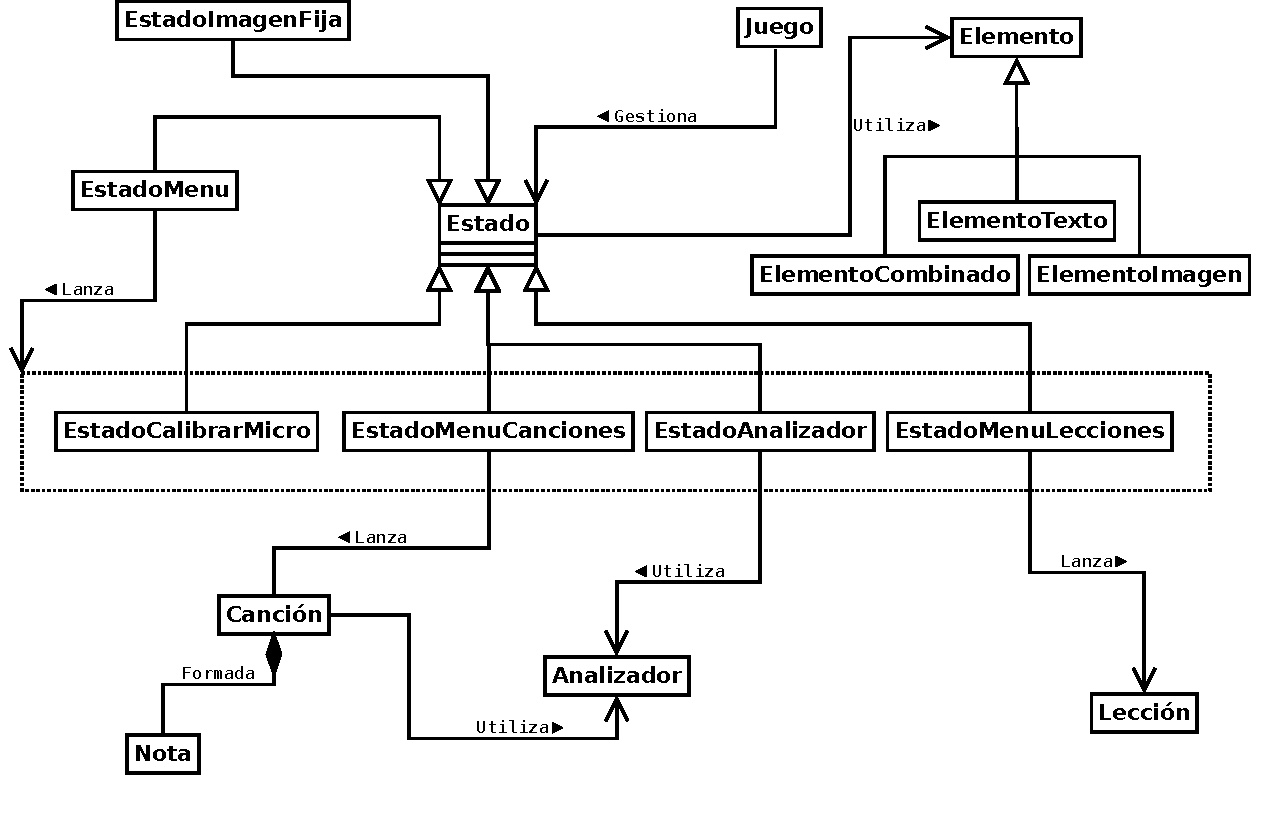
\includegraphics[angle=90]{4_analisis/imagen_diagrama_clases_conceptuales}
%   \caption{Diagrama de clases conceptuales}
% \end{figure}

% \pagebreak

%
\section{Modelo de comportamiento del sistema}
En esta sección vamos a especificar cómo se comporta el sistema en forma de dos
elementos fundamentales.
\begin{itemize}
\item En primer lugar, los \textbf{diagramas de secuencia} mostrarán el flujo de
  eventos entre los actores que participan en la aplicación.
\item En segundo lugar, los \textbf{contratos de las operaciones} detallarán las
  condiciones y efectos que tendrán lugar al ejecutarse las operaciones en el
  sistema.
\end{itemize}

\begin{nota}
  No se han reflejado, por triviales, los escenarios alternativos en los que el
  usuario cierra la ventana, correspondientes a los flujos \textit{*a} definidos
  en la sección anterior.
\end{nota}

\subsection{Caso de uso: inicio del juego}

\subsubsection{Escenario principal}

\begin{figure}[h!]
  \centering
  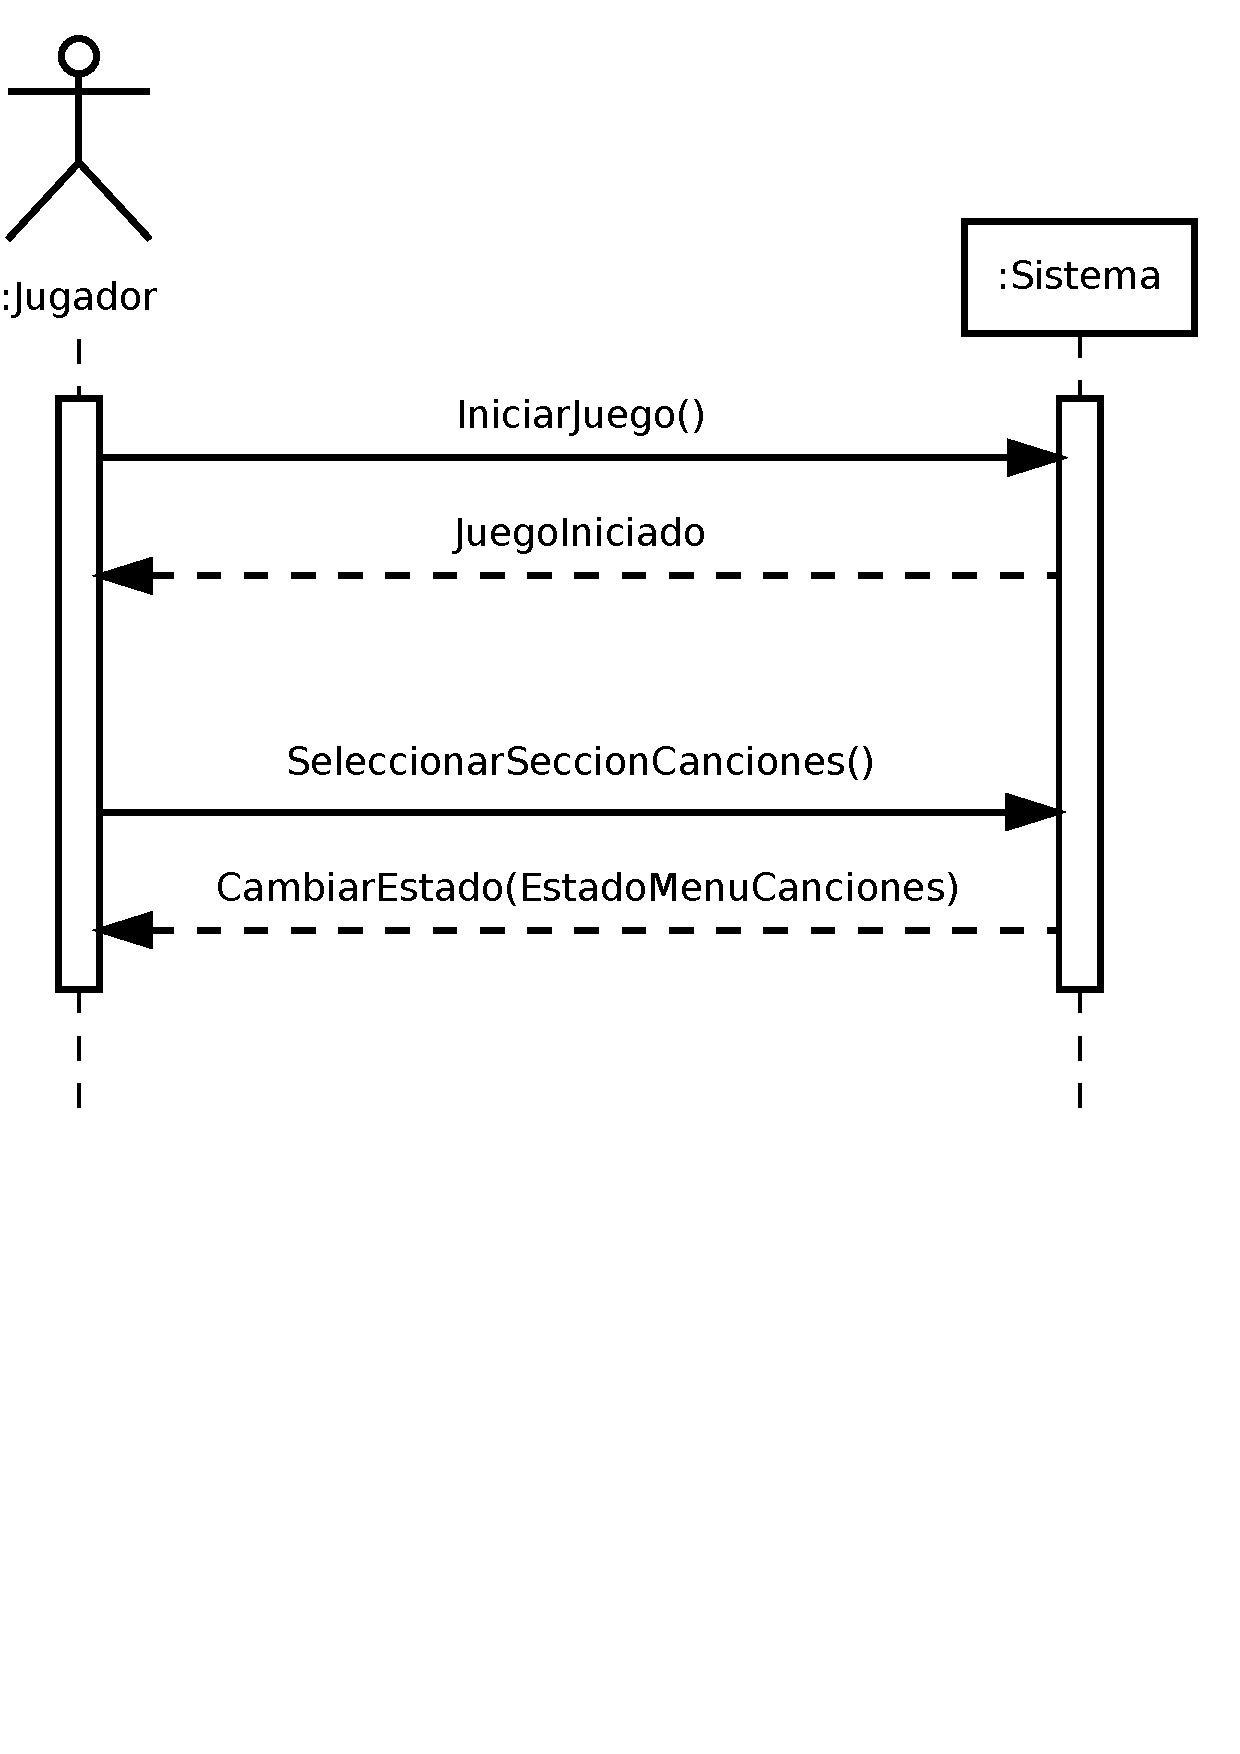
\includegraphics[trim=0cm 12cm 0cm 0cm, clip=true, width=0.5\textwidth]{4_analisis/diagsec_caso1_esc1}
  \caption{Diagrama de secuencia, incio del juego, escenario principal}
\end{figure}

\begin{description}
\item[Operación] IniciarJuego()
\item[Actores] \jugador\, \sistema\
\item[Responsabilidades] Cargar y lanzar la aplicación, mostrar los títulos de
  crédito y el menú principal.
\item[Precondiciones] Ninguna.
\item[Postcondiciones] $\quad$

  \begin{itemize}
  \item Se crea una instancia de la clase \textit{Juego}, que gestiona la
    creación y destrucción de los estados.
  \item Se crean y posteriormente destruyen dos estados
    \textit{EstadoImagenFija} para mostrar los títulos de crédito.
  \item Se crea y permanece un estado \textit{EstadoMenú}, que representa el
    menú principal de la aplicación.
  \end{itemize}

\end{description}

\begin{description}
\item[Operación] SeleccionarSeccionCanciones()
\item[Actores] \jugador\, \sistema\
\item[Responsabilidades] Esconder el menú principal y cargar el menú de
  selección de canciones.
\item[Precondiciones] $\quad$

  \begin{itemize}
  \item El estado actual es una instancia de \textit{EstadoMenú}.
  \end{itemize}

\item[Postcondiciones] Se destruye el estado \textit{EstadoMenú} y se carga
  \textit{EstadoMenúCanciones}.
\end{description}

\subsubsection{Escenario alternativo 4a}
\begin{figure}[h!]
  \centering
  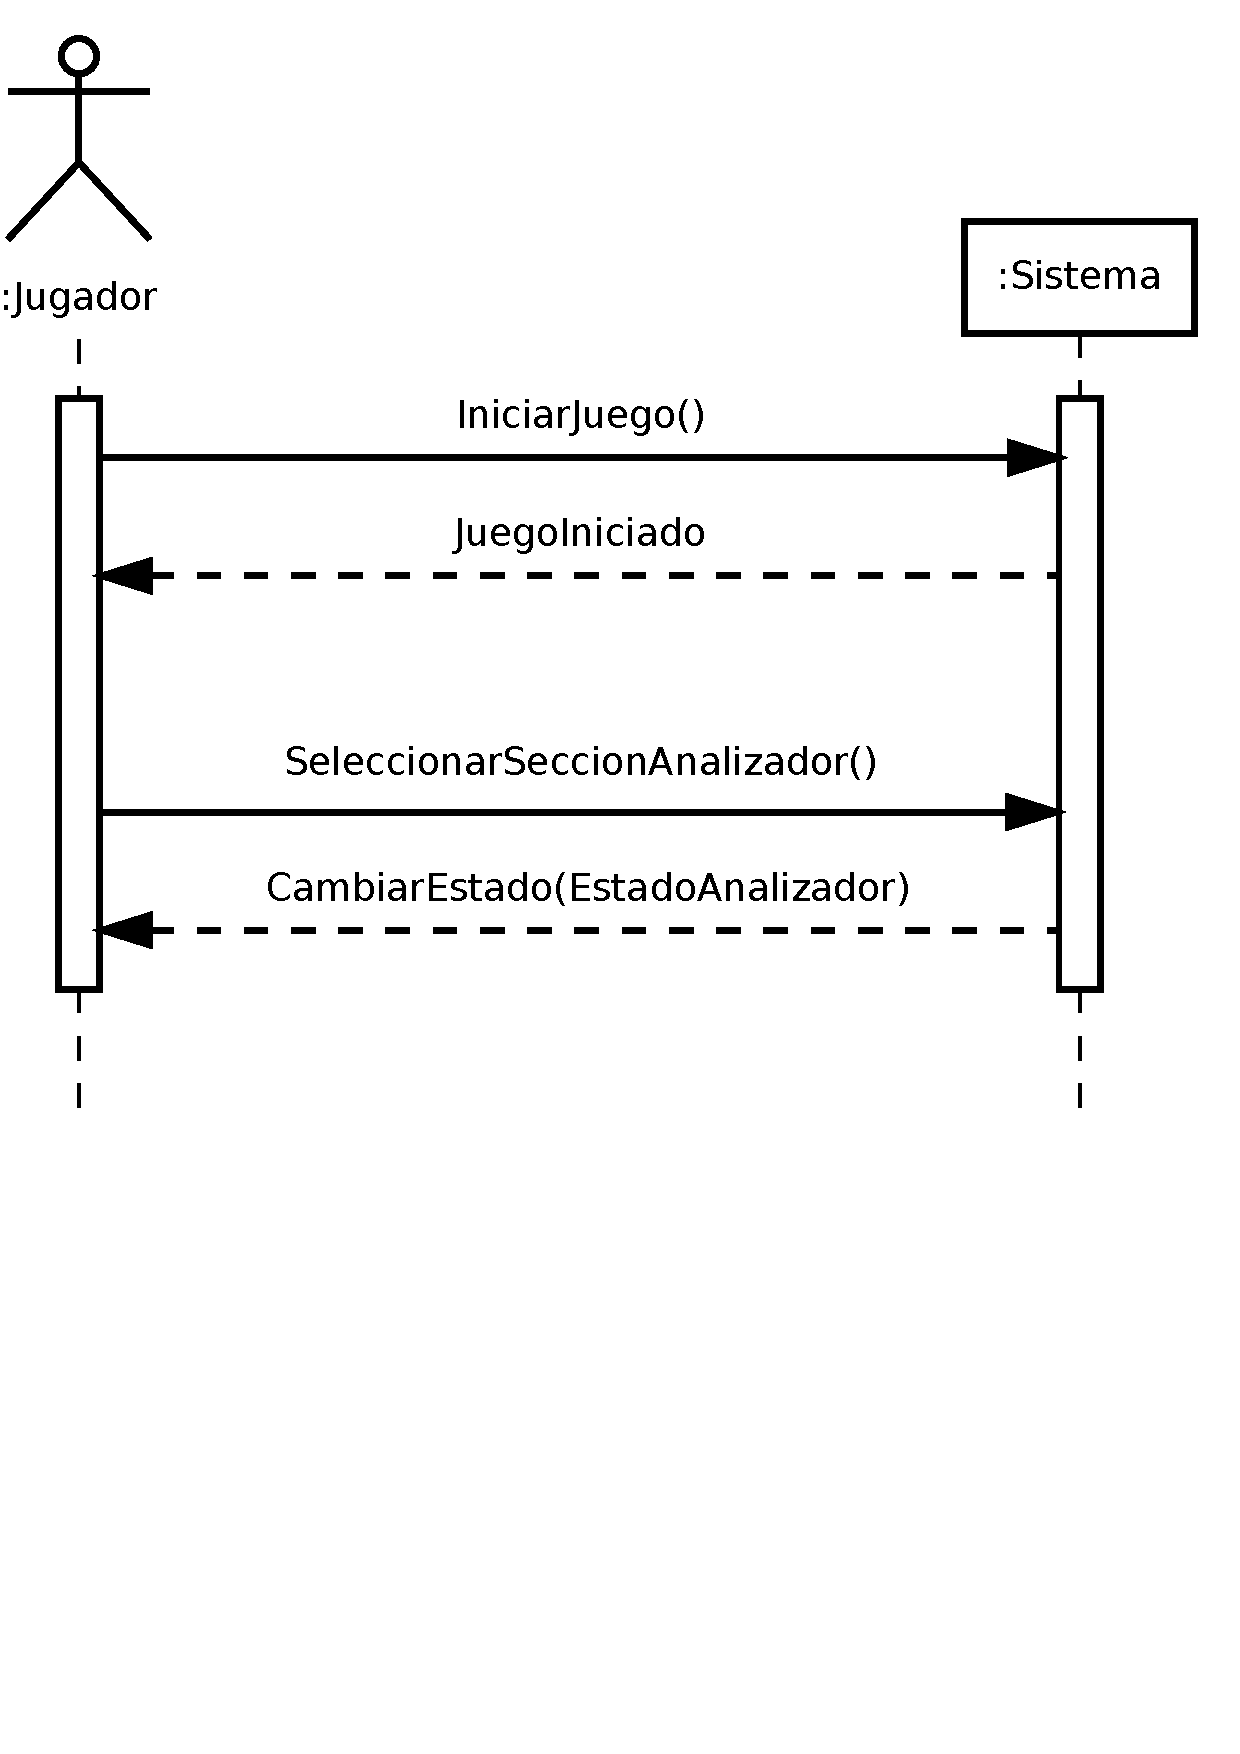
\includegraphics[trim=0cm 12cm 0cm 0cm, clip=true, width=0.5\textwidth]{4_analisis/diagsec_caso1_esc2}
  \caption{Diagrama de secuencia, incio del juego, escenario alternativo 4a}
\end{figure}

\begin{description}
\item[Operación] SeleccionarSeccionAnalizador()
\item[Actores] \jugador\, \sistema\
\item[Responsabilidades] Esconder el menú principal y cargar la sección de
  análisis de notas.
\item[Precondiciones] $\quad$
  \begin{itemize}
  \item El estado actual es una instancia de \textit{EstadoMenú}.
  \end{itemize}
\item[Postcondiciones] Se destruye el estado \textit{EstadoMenú} y se carga
  \textit{EstadoAnalizador}.
\end{description}

\subsubsection{Escenario alternativo 4b}
\begin{figure}[h!]
  \centering
  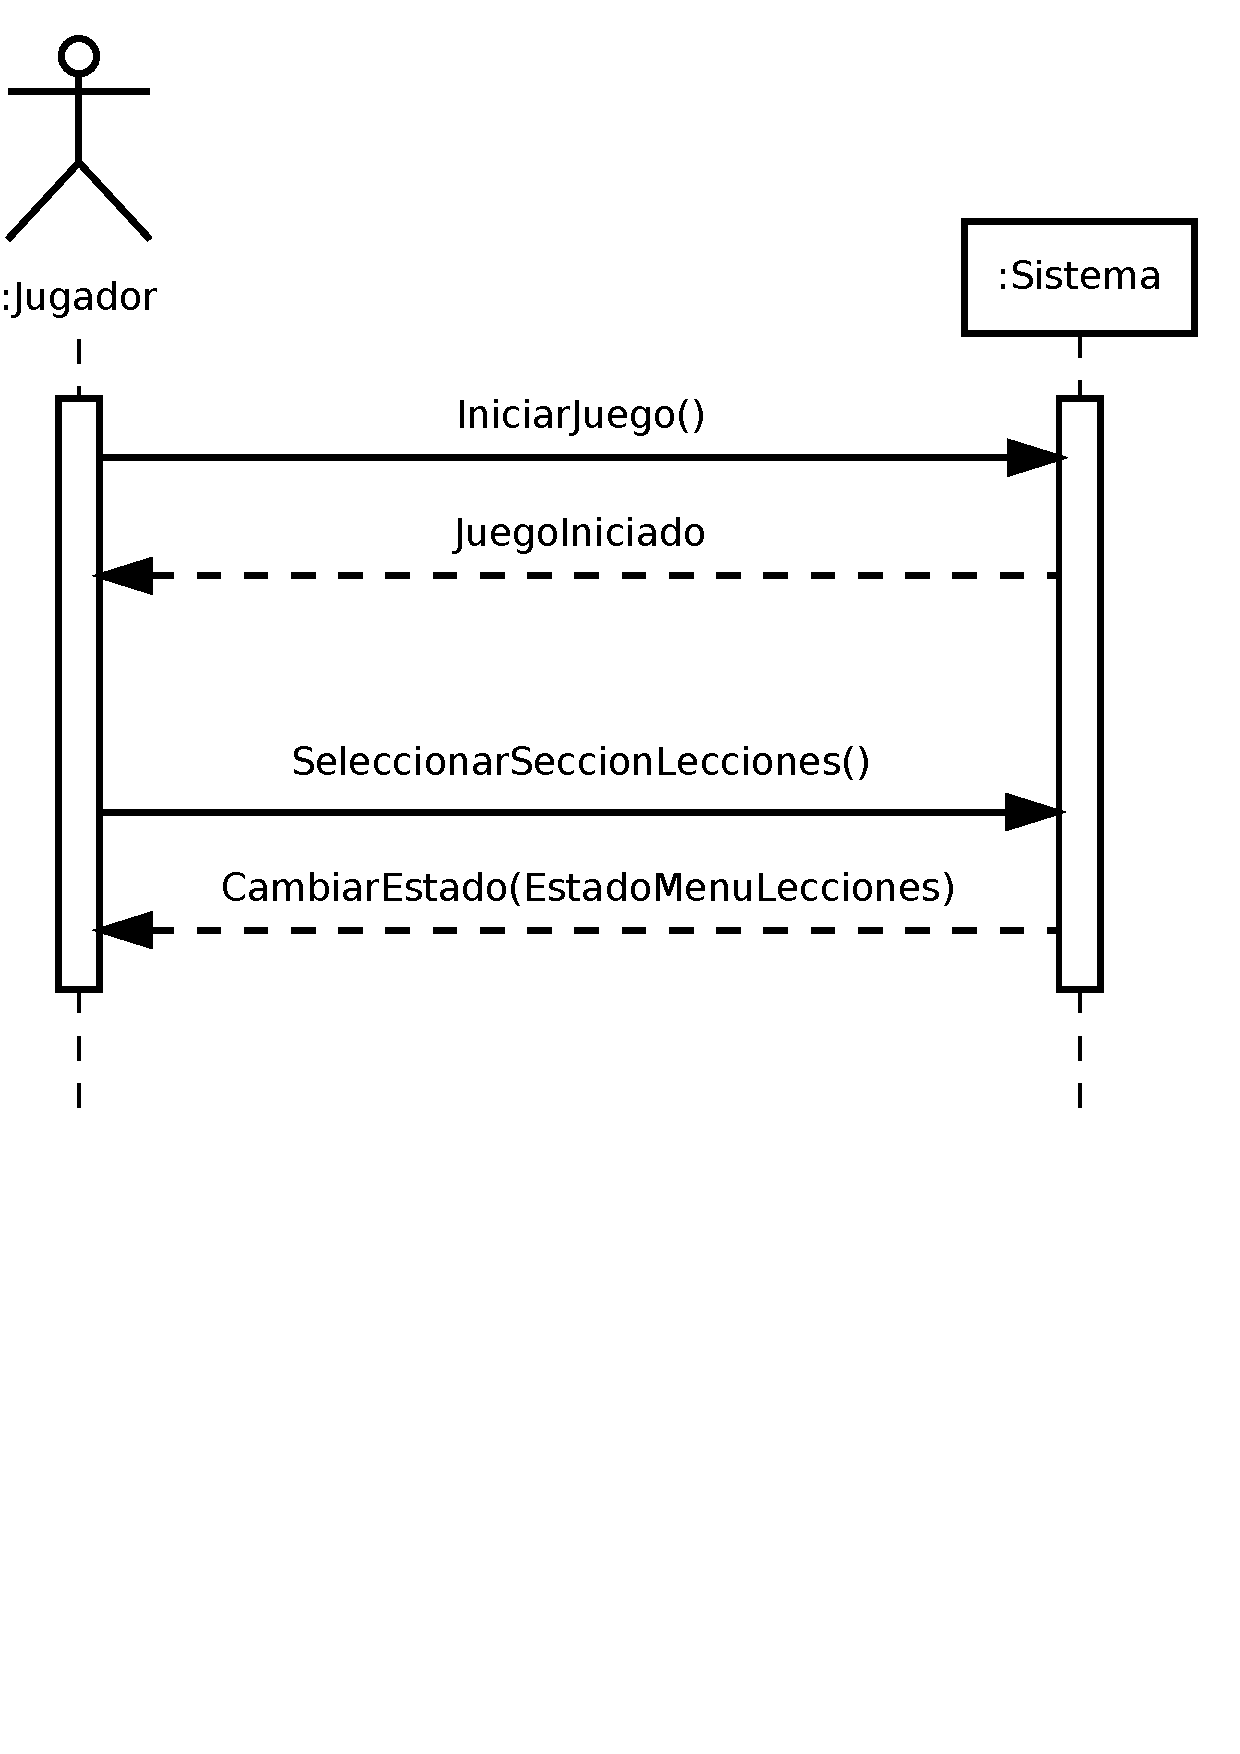
\includegraphics[trim=0cm 12cm 0cm 0cm, clip=true, width=0.5\textwidth]{4_analisis/diagsec_caso1_esc3}
  \caption{Diagrama de secuencia, incio del juego, escenario alternativo 4b}
\end{figure}

\begin{description}
\item[Operación] SeleccionarSeccionLecciones()
\item[Actores] \jugador\, \sistema\
\item[Responsabilidades] Esconder el menú principal y cargar la menú de
  selección de lecciones.
\item[Precondiciones] $\quad$
  \begin{itemize}
  \item El estado actual es una instancia de \textit{EstadoMenú}.
  \end{itemize}
\item[Postcondiciones] Se destruye el estado \textit{EstadoMenú} y se carga
  \textit{EstadoMenúLecciones}.
\end{description}

\subsubsection{Escenario alternativo 4c}
\begin{figure}[h!]
  \centering
  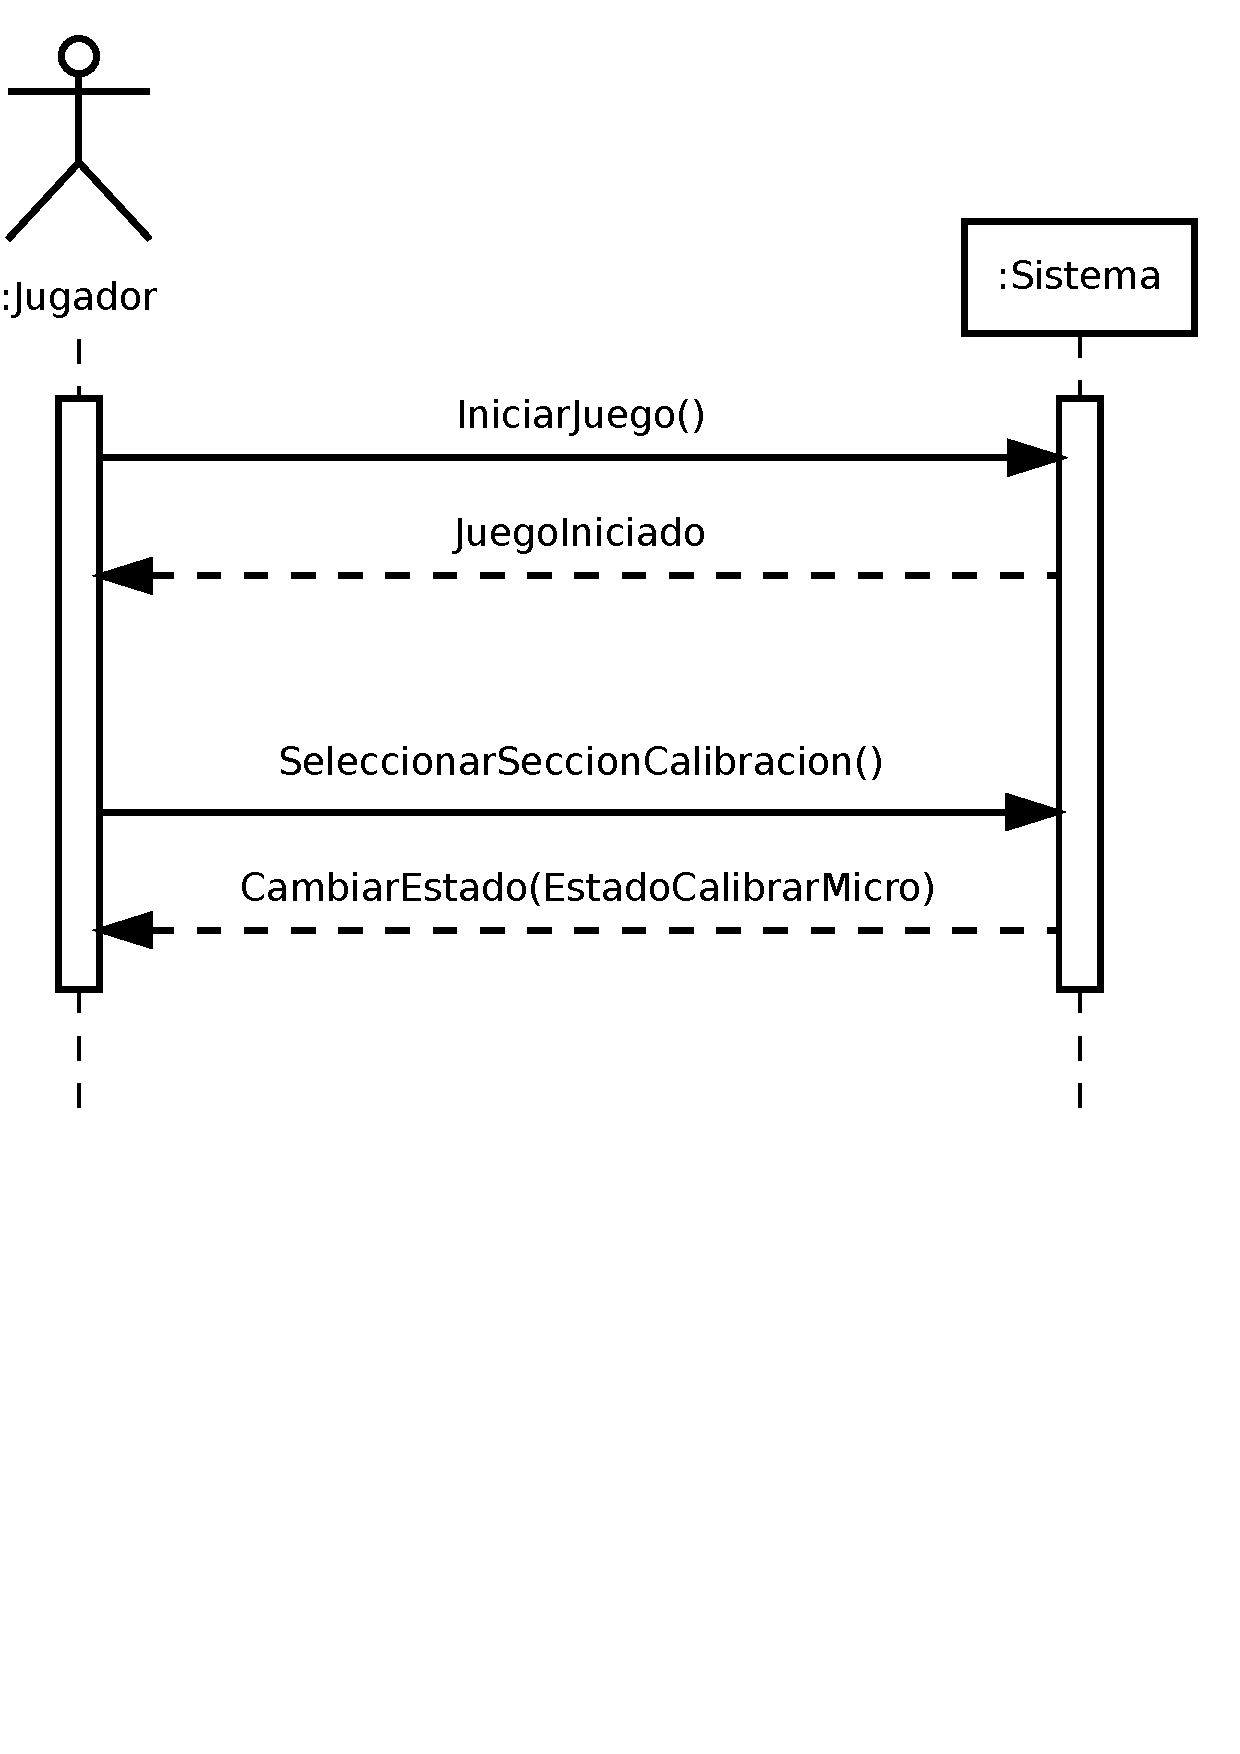
\includegraphics[trim=0cm 12cm 0cm 0cm, clip=true, width=0.5\textwidth]{4_analisis/diagsec_caso1_esc4}
  \caption{Diagrama de secuencia, incio del juego, escenario alternativo 4c}
\end{figure}

\begin{description}
\item[Operación] SeleccionarSeccionCalibracion()
\item[Actores] \jugador\, \sistema\
\item[Responsabilidades] Esconder el menú principal y cargar la sección de
  calibración de micrófono.
\item[Precondiciones] $\quad$
  \begin{itemize}
  \item El estado actual es una instancia de \textit{EstadoMenú}.
  \end{itemize}
\item[Postcondiciones] Se destruye el estado \textit{EstadoMenú} y se carga
  \textit{EstadoCalibrarMicro}.
\end{description}

\subsubsection{Escenario alternativo 4d}
\begin{figure}[h!]
  \centering
  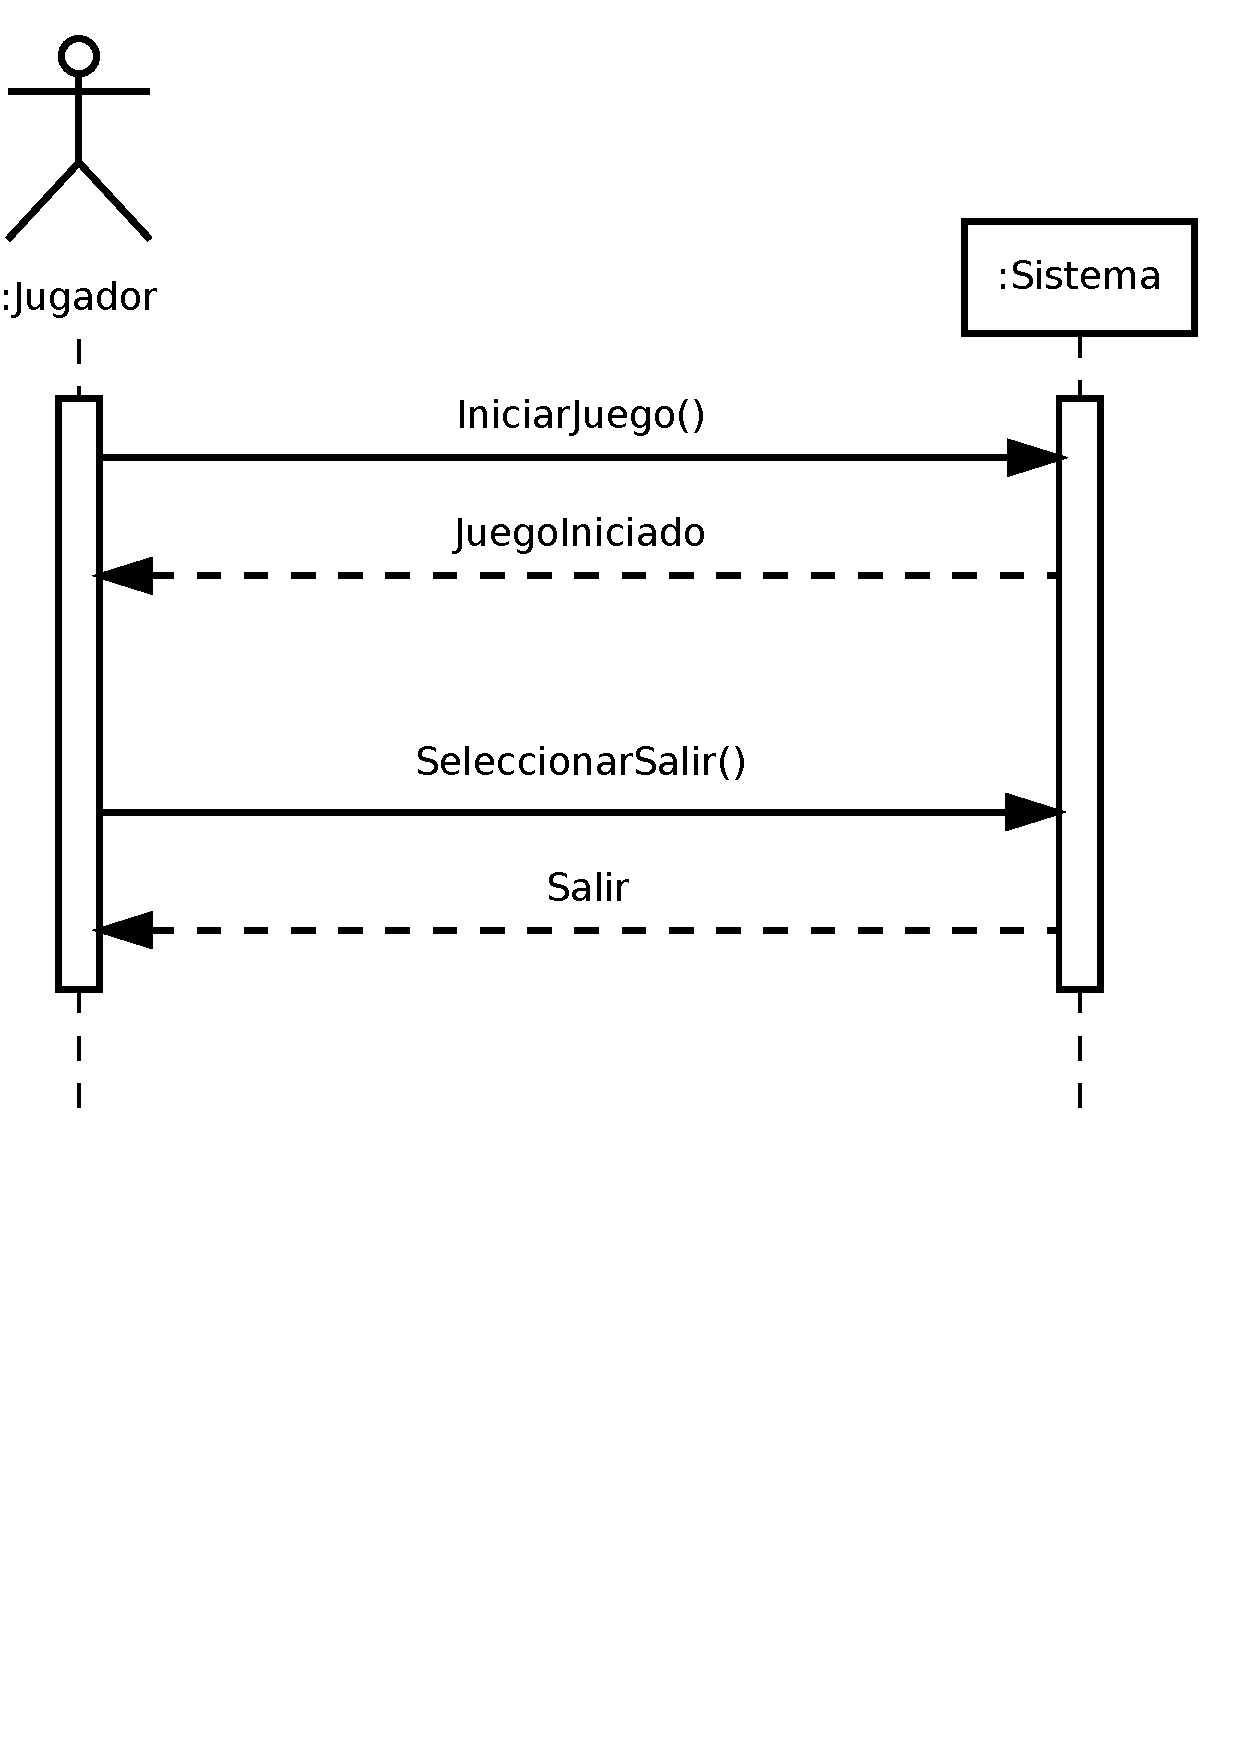
\includegraphics[trim=0cm 12cm 0cm 0cm, clip=true, width=0.5\textwidth]{4_analisis/diagsec_caso1_esc5}
  \caption{Diagrama de secuencia, incio del juego, escenario alternativo 4d}
\end{figure}

\begin{description}
\item[Operación] SeleccionarSalir()
\item[Actores] \jugador\, \sistema\
\item[Responsabilidades] Esconder el menú principal, descargar los recursos y
  cerrar la aplicación.
\item[Precondiciones] $\quad$
  \begin{itemize}
  \item El estado actual es una instancia de \textit{EstadoMenú}.
  \end{itemize}
\item[Postcondiciones] Se destruye el estado \textit{EstadoMenú}, se destruye la
  instancia de la clase \textit{Juego} y termina la ejecución de la aplicación.
\end{description}

\subsection{Selección de canción}

\subsubsection{Escenario principal}
\begin{figure}[h!]
  \centering
  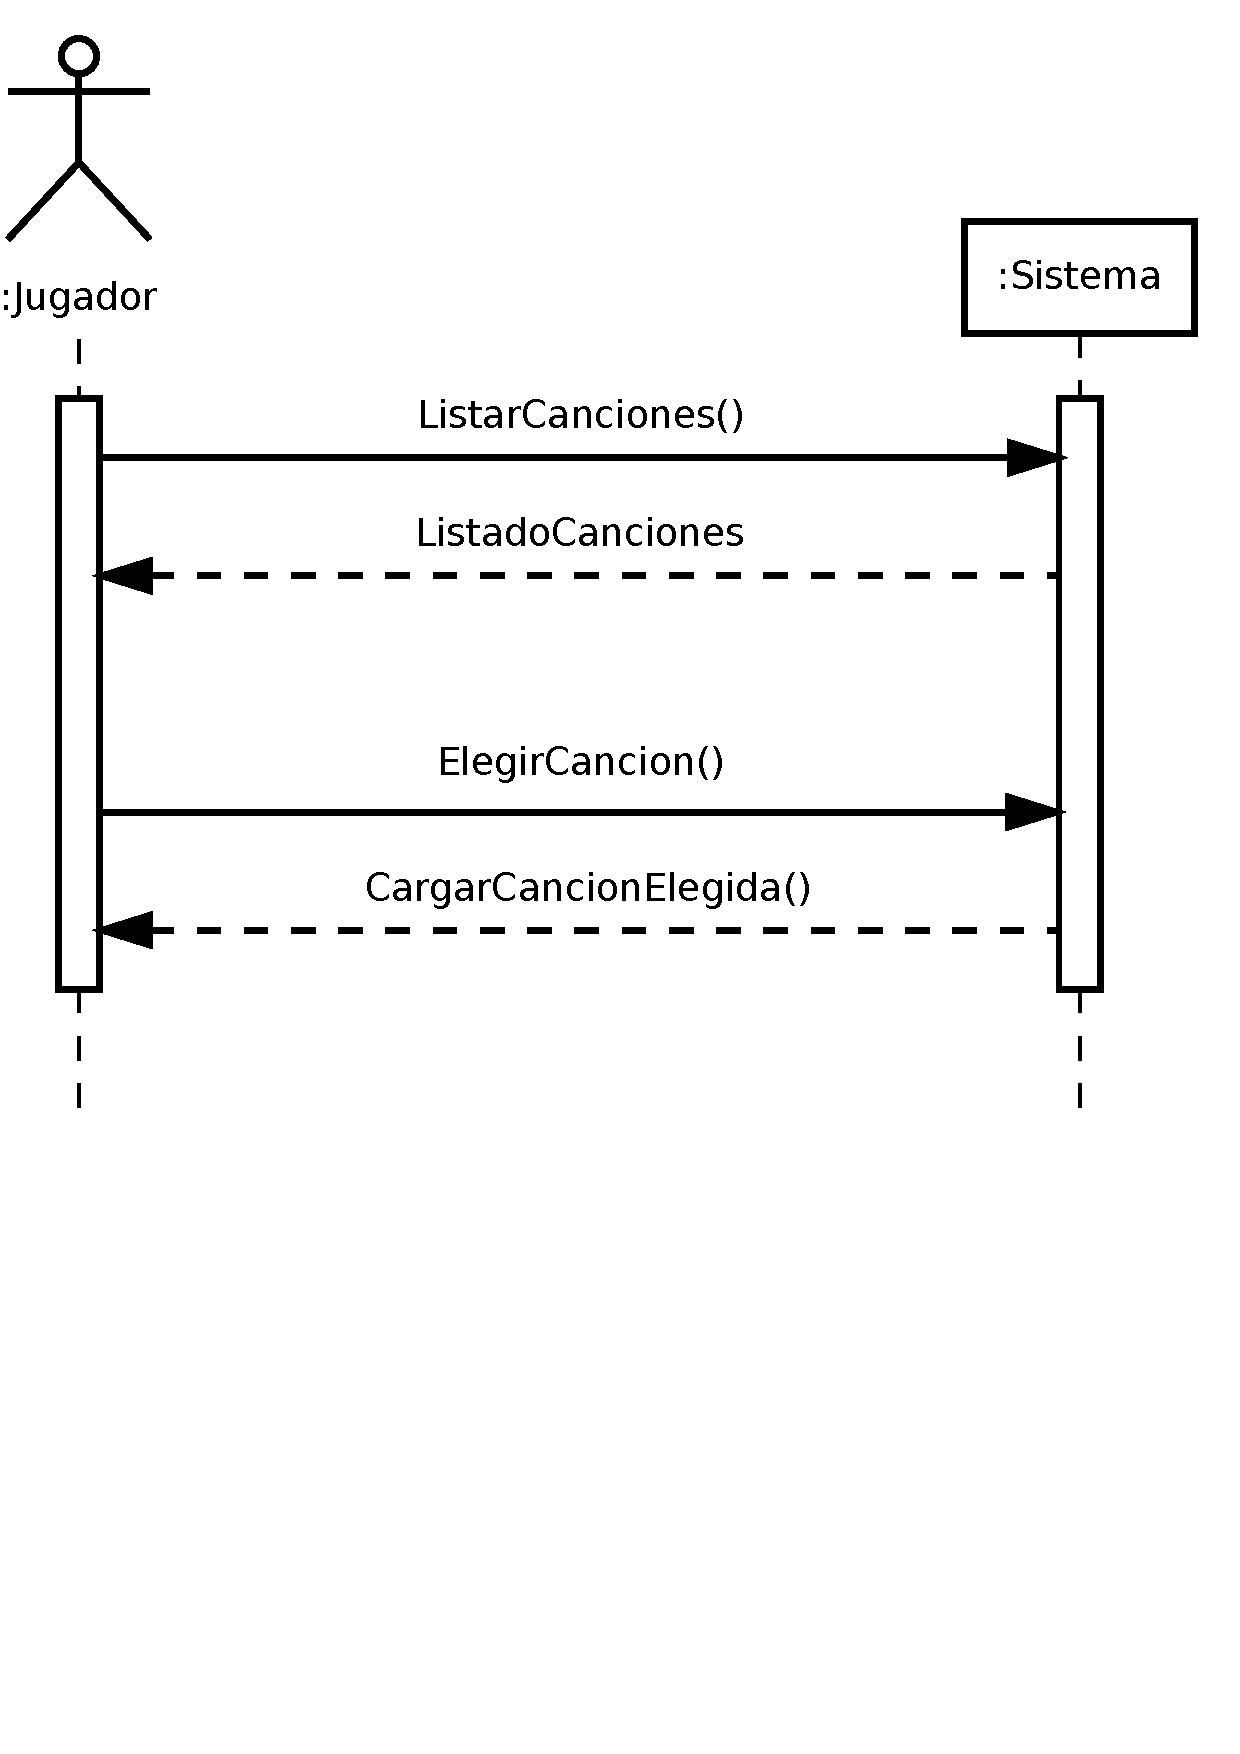
\includegraphics[trim=0cm 12cm 0cm 0cm, clip=true, width=0.5\textwidth]{4_analisis/diagsec_caso2_esc1}
  \caption{Diagrama de secuencia, selección de canción, escenario principal}
\end{figure}

\begin{description}
\item[Operación] ListarCanciones()
\item[Actores] \jugador\, \sistema\
\item[Responsabilidades] Cargar y mostrar la lista de canciones cargadas en el
  sistema.
\item[Precondiciones] Se ordenó la carga del estado \textit{EstadoMenuCanción}
\item[Postcondiciones] $\quad$
  \begin{itemize}
  \item El estado actual es una instancia de \textit{EstadoMenuCanción}.
  \item Se ha cargado la lista de canciones y se muestra en pantalla.
  \end{itemize}
\end{description}

\begin{description}
\item[Operación] ElegirCanción()
\item[Actores] \jugador\, \sistema\
\item[Responsabilidades] Cargar la canción que el usuario ha elegido para
  interpretar.
\item[Precondiciones] Existe una lista de canciones cargada de entre las que el
  usuario ha elegido una.
\item[Postcondiciones] $\quad$
  \begin{itemize}
  \item Se carga la canción indicada.
  \item Se oculta la lista de canciones.
  \item Se pasa a un sub-estado de interpretación de canción.
  \end{itemize}
\end{description}
\subsubsection{Escenario alternativo 3a}
\begin{figure}[h!]
  \centering
  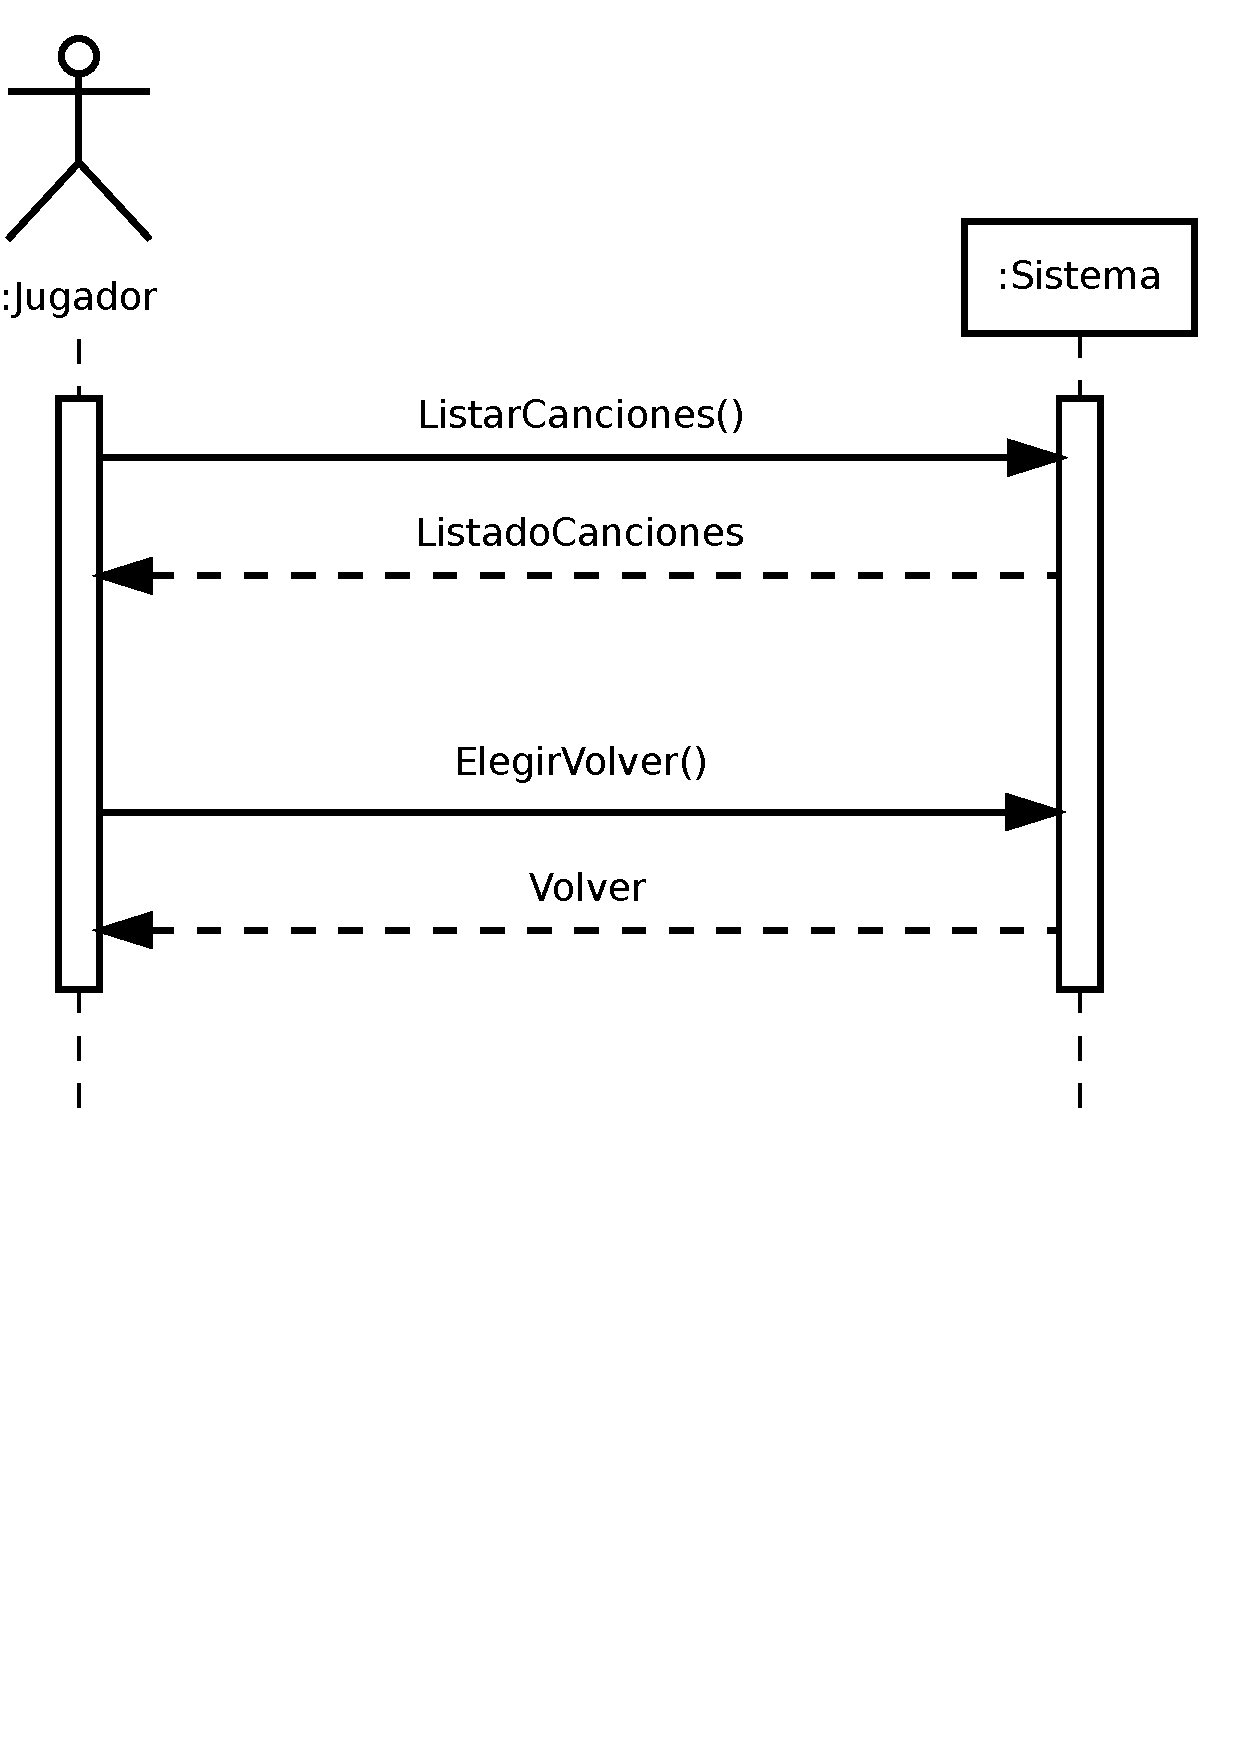
\includegraphics[trim=0cm 12cm 0cm 0cm, clip=true, width=0.5\textwidth]{4_analisis/diagsec_caso2_esc2}
  \caption{Diagrama de secuencia, selección de canción, escenario alternativo 3a}
\end{figure}
\begin{description}
\item[Operación] ElegirVolver()
\item[Actores] \jugador\, \sistema\
\item[Responsabilidades] Descargar la sección actual y volver al menú anterior.
\item[Precondiciones] El estado actual es una instancia de \textit{EstadoMenuCanción}.
\item[Postcondiciones] $\quad$
  \begin{itemize}
  \item El estado instancia de \textit{EstadoMenuCanción} queda descargado.
  \item Se carga y se muestra \textit{EstadoMenú}.
  \end{itemize}
\end{description}

\subsection{Interpretación de canción}
\begin{nota}
  No se reflejan los escenarios alternativos al estar englobados en la operación
  \textit{InteractuarConFlauta}.
\end{nota}

\subsubsection{Escenario principal}
\begin{figure}[h!]
  \centering
  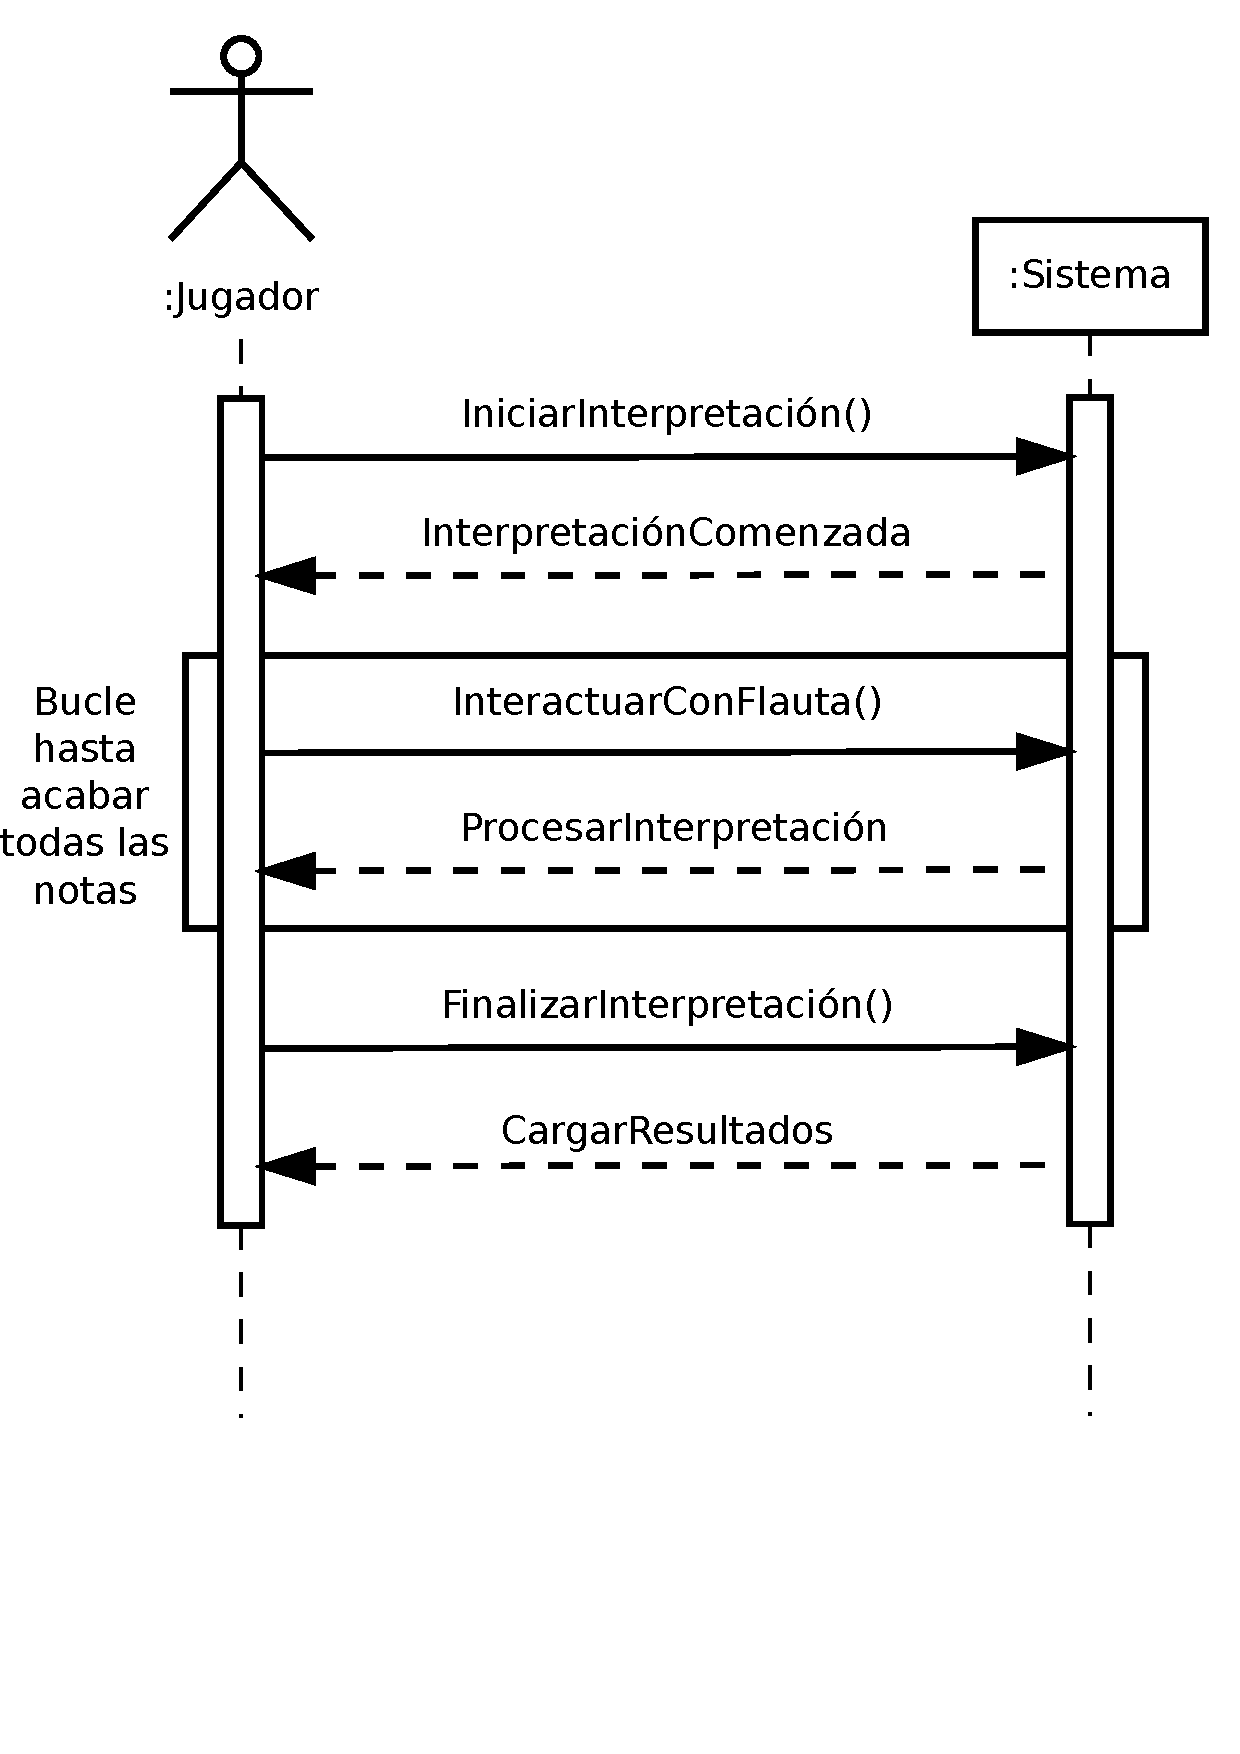
\includegraphics[trim=0cm 8cm 0cm 0cm, clip=true, width=0.5\textwidth]{4_analisis/diagsec_caso3}
  \caption{Diagrama de secuencia, interpretación de canción, escenario principal}
\end{figure}

\begin{description}
\item[Operación] IniciarInterpretación()
\item[Actores] \jugador\, \sistema\
\item[Responsabilidades] Parsear el fichero de canción, cargar la interfaz y
  comenzar la interpretación.
\item[Precondiciones] El usuario ha elegido una canción en el estado anterior.
\item[Postcondiciones] $\quad$
  \begin{itemize}
  \item Se muestra la interfaz de interpretación de canción.
  \item El fichero de canción queda cargado e interpretado, instanciando los
    elementos de la clase \textit{Nota} que sean necesarios.
  \item Comienza la interpretación
  \end{itemize}
\end{description}

\begin{description}
\item[Operación] InteractuarConFlauta()
\item[Actores] \jugador\, \sistema\
\item[Responsabilidades] El \jugador\ interactúa con el sistema mediante la
  flauta a través del micrófono, y el \sistema\ analiza los datos y muestra una
  respuesta en pantalla.
\item[Precondiciones] $\quad$
  \begin{itemize}
  \item La interpretación ha comenzado.
  \item El micrófono está correctamente configurado.
  \end{itemize}
\item[Postcondiciones] $\quad$
  \begin{itemize}
  \item El sistema captura y analiza los datos de audio.
  \item Según el análisis, el sistema responde de una forma u otra (según los
    escenarios alternativos 3a, 4a y 5a del caso de uso \textit{interpretación
      de canción}).
  \end{itemize}
\end{description}

\begin{description}
\item[Operación] FinalizarInterpretación()
\item[Actores] \jugador\, \sistema\
\item[Responsabilidades] Descargar la pantalla de interpretación, descargar la
  canción y finalizar la interpretación.
\item[Precondiciones] Todas las notas se han interpretado.
\item[Postcondiciones] $\quad$
  \begin{itemize}
  \item Se descarga la \textit{Canción} actual.
  \item Se ocultan los elementos de la interfaz de interpretación.
  \item Se lanza la sección de puntuación.
  \end{itemize}
\end{description}


\subsection{Resultados de interpretación}

\subsubsection{Escenario principal}
\begin{figure}[h!]
  \centering
  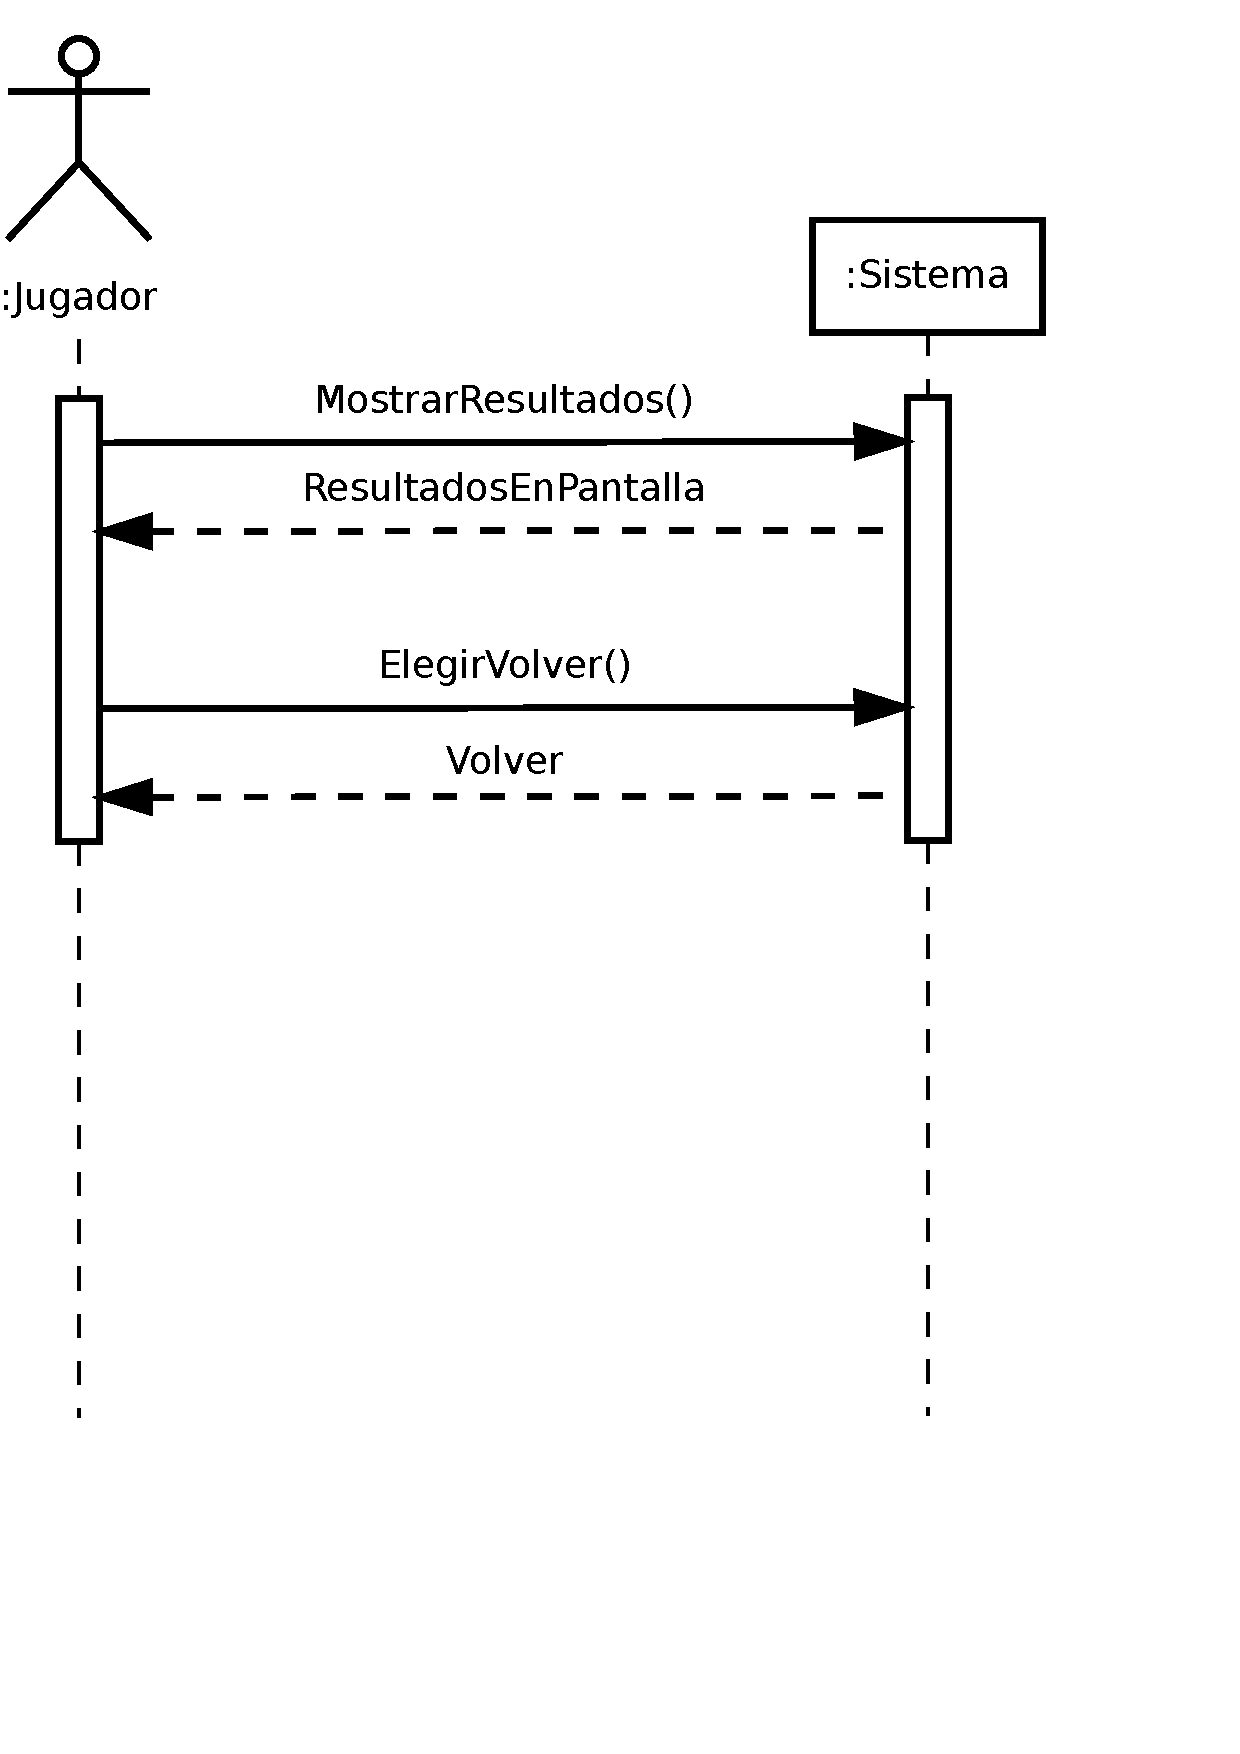
\includegraphics[trim=0cm 12cm 0cm 0cm, clip=true, width=0.5\textwidth]{4_analisis/diagsec_caso4}
  \caption{Diagrama de secuencia, resultados de interpretación, escenario principal}
\end{figure}

\begin{description}
\item[Operación] MostrarResultados()
\item[Actores] \jugador\, \sistema\
\item[Responsabilidades] Interpretar los resultados de la interpretación y
  mostrar los resultados en pantalla.
\item[Precondiciones] El \jugador\ ha concluído satisfactoriamente una
  interpretación completa de una canción, obteniendo una suma de puntos $X$.
\item[Postcondiciones] Mostrar en pantalla los resultados en forma de porcentaje
  de aciertos, y un mensaje según aquél.
\end{description}

\begin{description}
\item[Operación] ElegirVolver()
\item[Actores] \jugador\, \sistema\
\item[Responsabilidades] Descargar la sección actual y volver al menú anterior.
\item[Precondiciones] $\quad$
  \begin{itemize}
  \item La aplicación se encuentra en la pantalla de muestra de resultados.
  \item El usuario ha pulsado la tecla \texttt{escape} o el botón \textit{volver}.
  \end{itemize}
\item[Postcondiciones] $\quad$
  \begin{itemize}
  \item Se descargan todos los datos referentes a la canción actual.
  \item Se carga y se muestra \textit{EstadoMenúCanciones}.
  \end{itemize}
\end{description}

\subsection{Analizador de notas}

\begin{nota}
  No se reflejan los escenarios alternativos al estar englobados en la operación
  \textit{InteractuarConFlauta}.
\end{nota}

\subsubsection{Escenario principal}
\begin{figure}[h!]
  \centering
  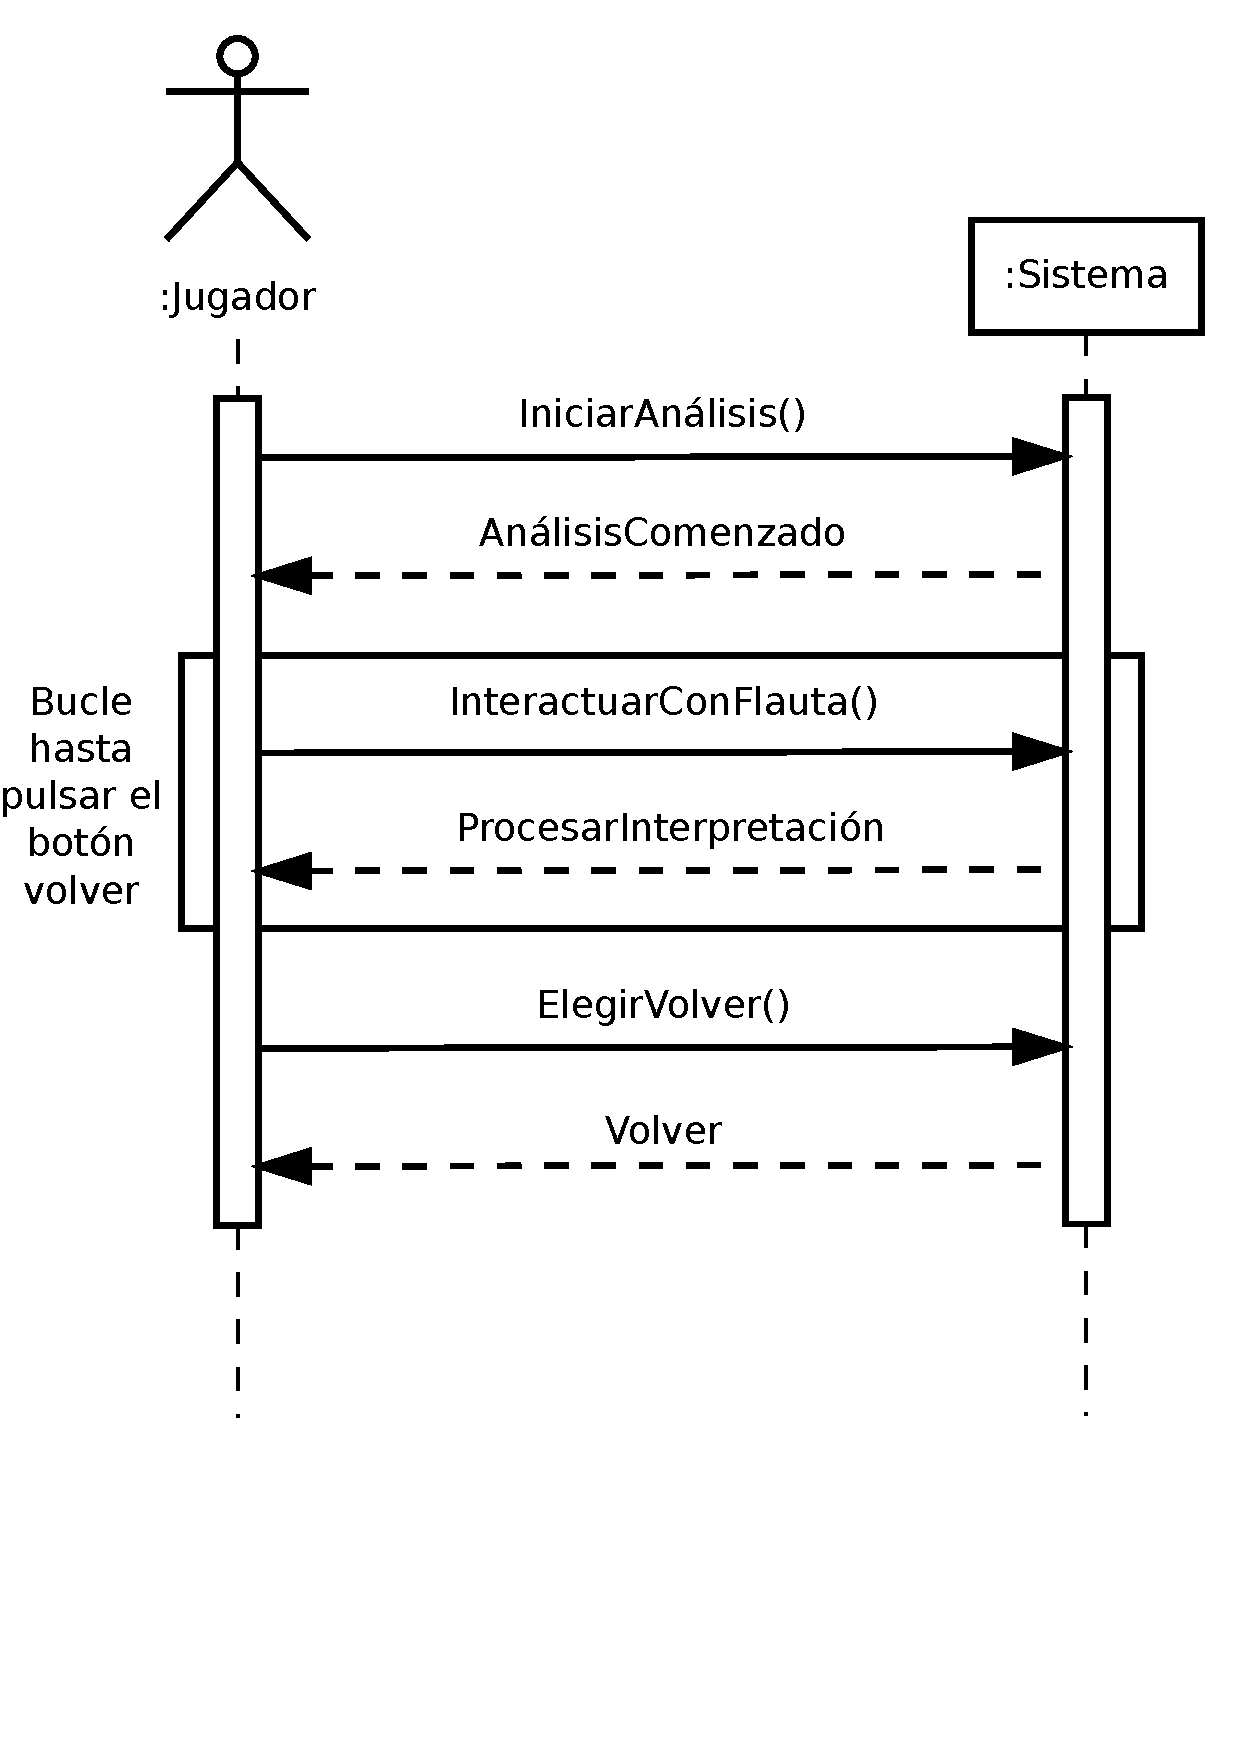
\includegraphics[trim=0cm 8cm 0cm 0cm, clip=true, width=0.5\textwidth]{4_analisis/diagsec_caso5}
  \caption{Diagrama de secuencia, interpretación de canción, escenario principal}
\end{figure}

\begin{description}
\item[Operación] IniciarAnálisis
\item[Actores] \jugador\, \sistema\
\item[Responsabilidades] Cargar la interfaz e iniciar el análisis de notas.
\item[Precondiciones] El usuario eligió la sección \textit{Analizador de notas}
  en el menú principal.
\item[Postcondiciones] $\quad$
  \begin{itemize}
  \item Aparece la interfaz del analizador de notas.
  \item Se inicia el análisis de notas
  \end{itemize}
\end{description}

\begin{description}
\item[Operación] InteractuarConFlauta
\item[Actores] \jugador\, \sistema\
\item[Responsabilidades] El \jugador\ toca notas en la flauta y el \sistema\
  captura y reconoce el audio, indicando la nota tocada en pantalla.

\item[Precondiciones] Se ha iniciado el análisis.

\item[Postcondiciones] $\quad$
  \begin{itemize}
  \item El \sistema\ recoge y analiza el sonido que emite la flauta del \jugador.
  \item El \sistema\ representa en pantalla la nota identificada, o no muestra
    nada en caso de identificación defectuosa.
  \end{itemize}
\end{description}

% \begin{description}
% \item[Operación] ElegirVolver()
% \item[Actores] \jugador\, \sistema\
% \item[Responsabilidades] Descargar la sección actual y volver al menú anterior.
% \item[Precondiciones] $\quad$
%   \begin{itemize}
%   \item El estado actual es una instancia de \textit{EstadoAnalizador}.
%   \item Hay un análisis en curso.  
%   \end{itemize}
  
% \item[Postcondiciones] $\quad$
%   \begin{itemize}
%   \item Concluye el análisis actual.
%   \item Se destruye el estado.
%   \item Se carga y se muestra \textit{EstadoMenú}.
%   \end{itemize}
% \end{description}

\subsection{Calibración de micrófono}

\subsubsection{Escenario principal}
\begin{figure}[h!]
  \centering
  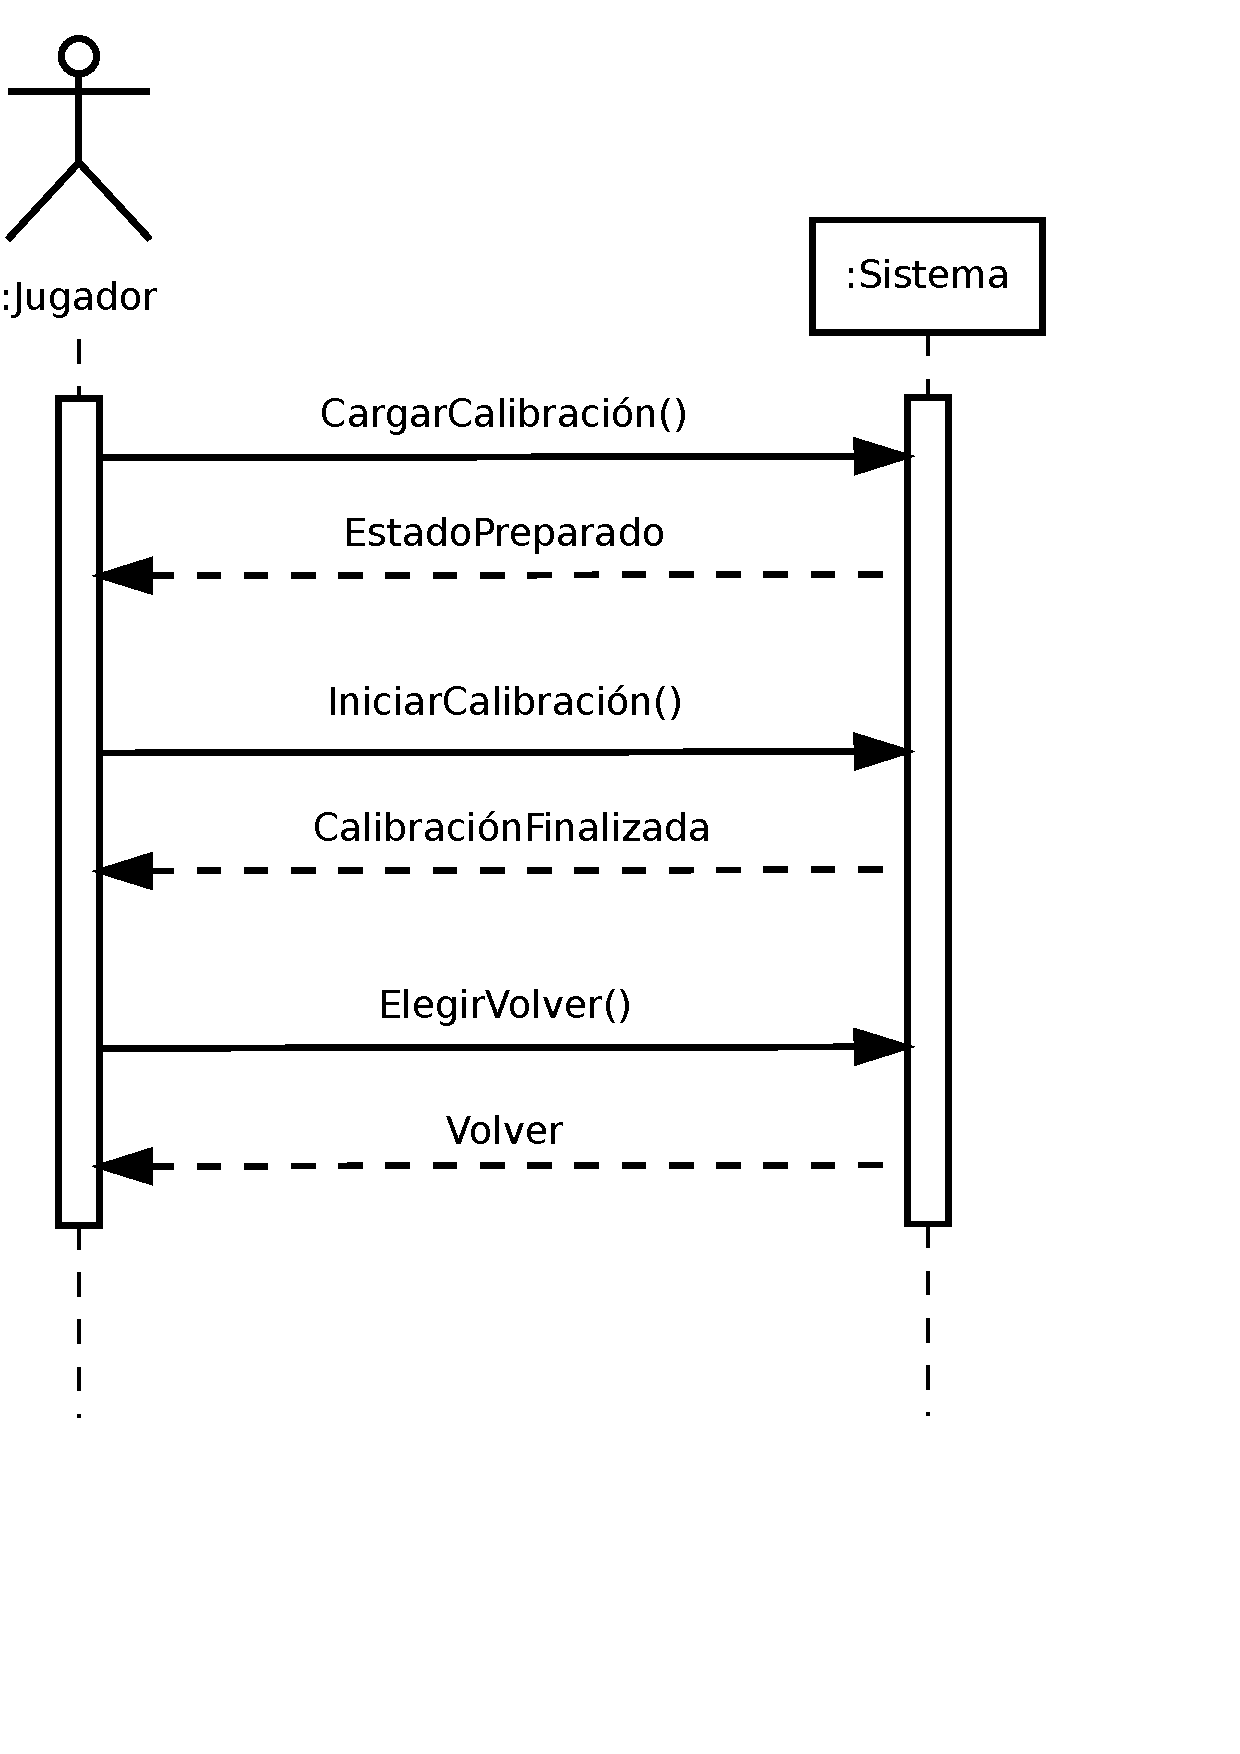
\includegraphics[trim=0cm 8cm 0cm 0cm, clip=true, width=0.5\textwidth]{4_analisis/diagsec_caso6_esc1}
  \caption{Diagrama de secuencia, calibración de micrófono, escenario principal}
\end{figure}

\begin{description}
\item[Operación] CargarCalibración()
\item[Actores] \jugador\, \sistema\
\item[Responsabilidades] Cargar la sección y preparar el sistema para comenzar
  la calibración del micrófono.
\item[Precondiciones] El usuario ha elegido en el menú principal la opción
  \textit{Calibrar micrófono}.
\item[Postcondiciones] La sección está cargada y la calibración lista para
  iniciarse.
\end{description}

\begin{description}
\item[Operación] CalibrarMicrófono()
\item[Actores] \jugador\, \sistema\
\item[Responsabilidades] Llevar a cabo la calibración correcta del micrófono.
\item[Precondiciones] El usuario ha lanzado la calibración del micrófono.
\item[Postcondiciones] $\quad$
  \begin{itemize}
  \item Se cierra el sistema de sonido.
  \item Se obtiene un valor umbral de ruido ambiente, fruto de una calibración
    exitosa.
  \end{itemize}
\end{description}

\begin{description}
\item[Operación] ElegirVolver()
\item[Actores] \jugador\, \sistema\
\item[Responsabilidades] Descargar la sección actual y volver al menú anterior.
\item[Precondiciones] $\quad$
  \begin{itemize}
  \item La calibración ha concluído exitosamente.
  \item El usuario ha pulsado la tecla \texttt{escape} o el botón \textit{volver}.
  \end{itemize}
\item[Postcondiciones] $\quad$
  \begin{itemize}
  \item Se descarga la sección actual.
  \item Se carga y se muestra \textit{EstadoMenúCanciones}.
  \end{itemize}
\end{description}

\subsubsection{Escenario alternativo 5a}
\begin{figure}[h!]
  \centering
  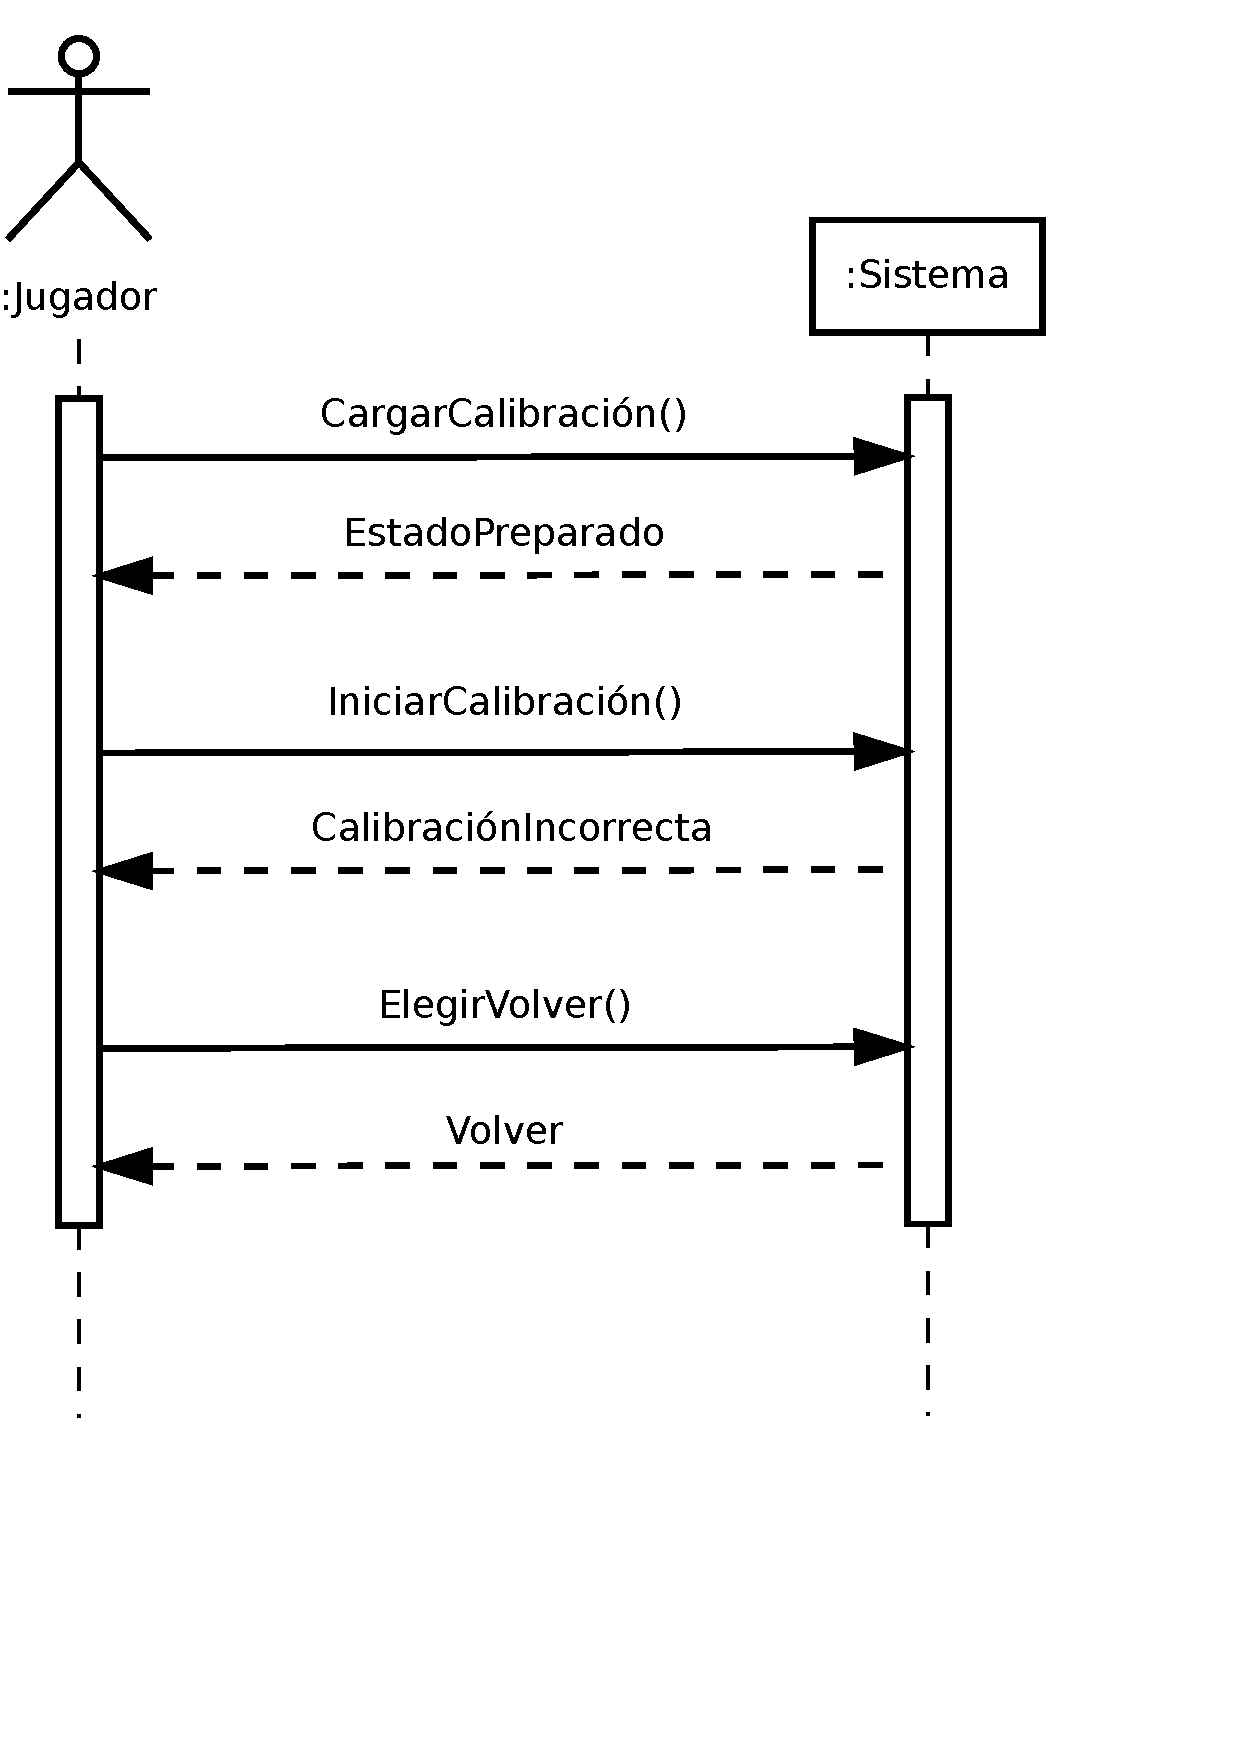
\includegraphics[trim=0cm 8cm 0cm 0cm, clip=true, width=0.5\textwidth]{4_analisis/diagsec_caso6_esc2}
  \caption{Diagrama de secuencia, calibración de micrófono, escenario principal}
\end{figure}
\begin{description}
\item[Operación] CalibrarMicrófono()
\item[Actores] \jugador\, \sistema\
\item[Responsabilidades] Llevar a cabo la calibración correcta del micrófono.
\item[Precondiciones] El usuario ha lanzado la calibración del micrófono.
\item[Postcondiciones] $\quad$
  \begin{itemize}
  \item Se cierra el sistema de sonido.
  \item La calibración ha fallado.
  \item No se obtiene valor umbral de ruido ambiental.
  \end{itemize}
\end{description}

\subsection{Selección de lecciones}

\subsubsection{Escenario principal}
\begin{figure}[h!]
  \centering
  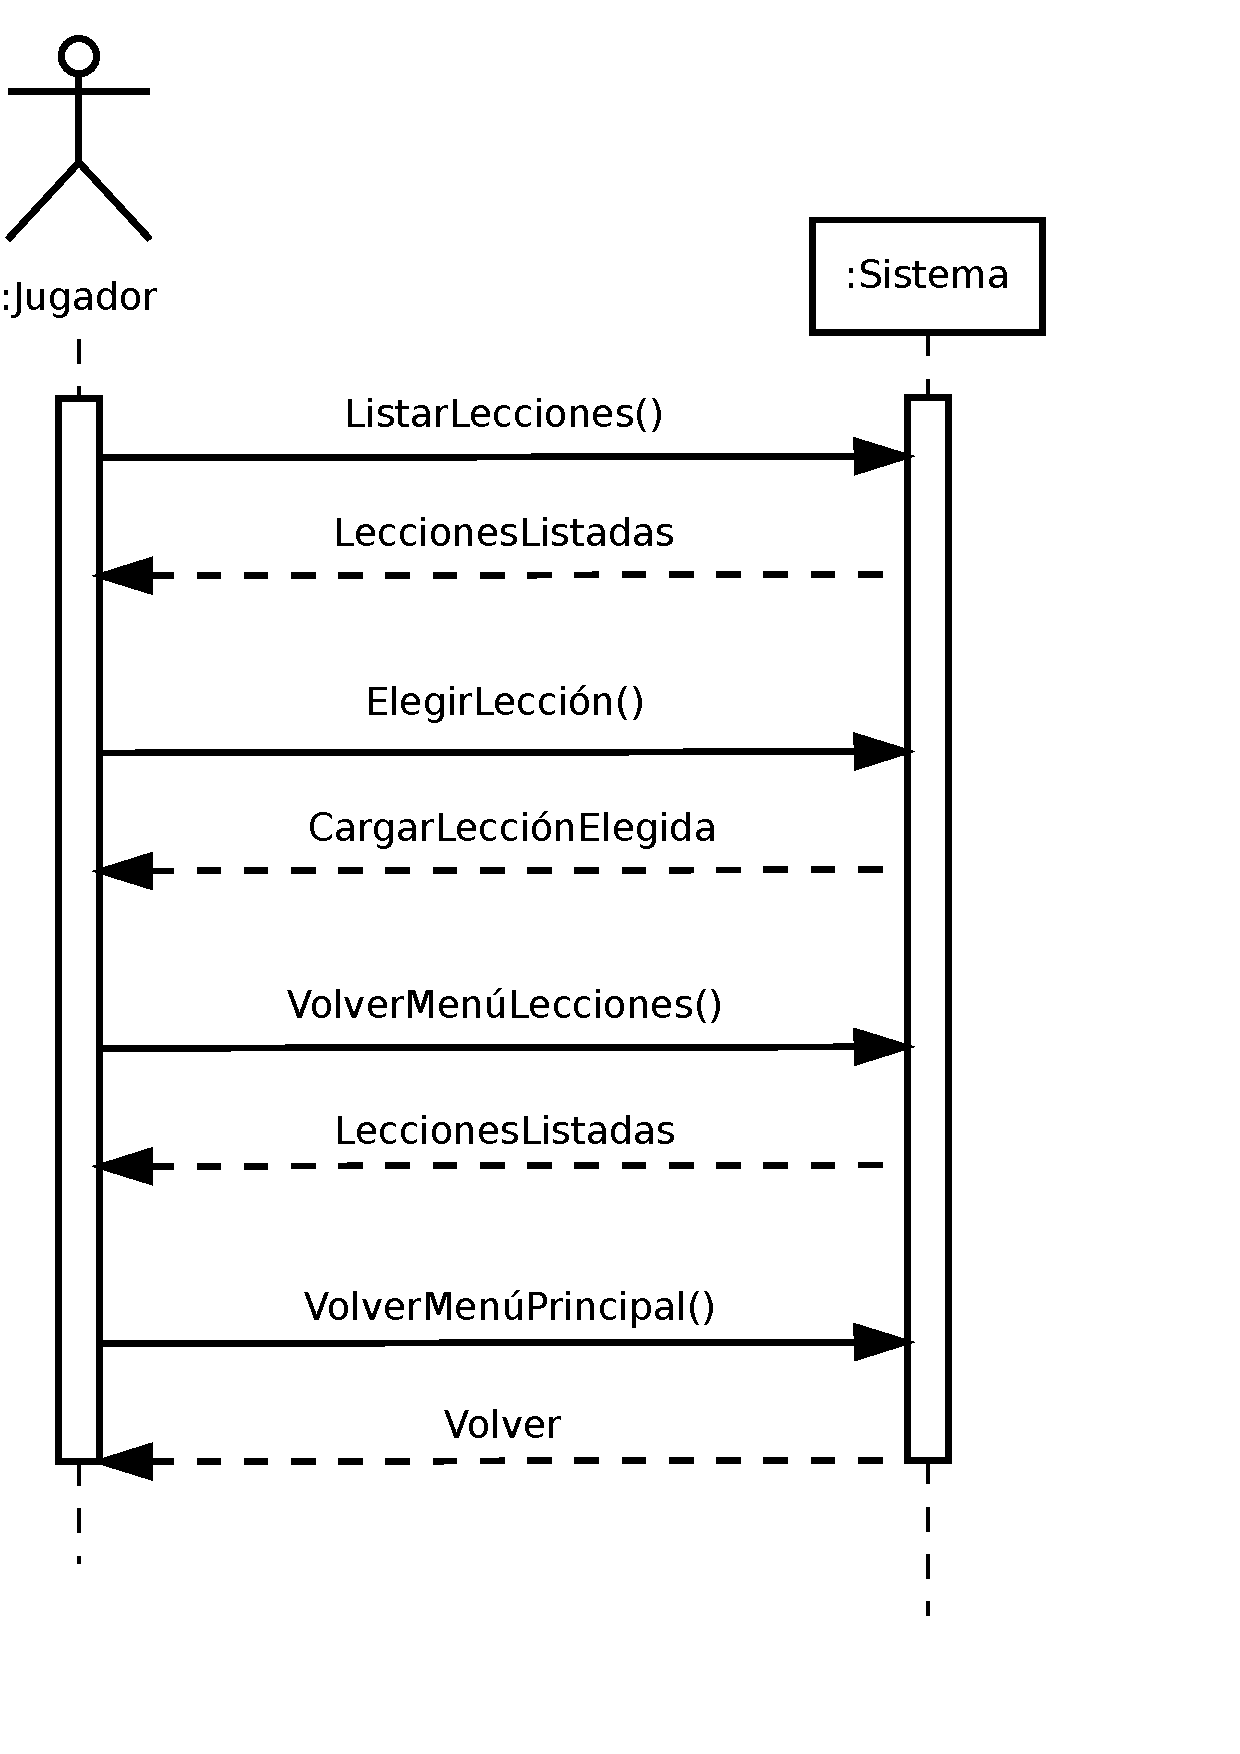
\includegraphics[trim=0cm 4cm 0cm 0cm, clip=true, width=0.5\textwidth]{4_analisis/diagsec_caso7_esc1}
  \caption{Diagrama de secuencia, selección delecciones, escenario principal}
\end{figure}


\begin{description}
\item[Operación] ListarLecciones()
\item[Actores] \jugador\, \sistema\
\item[Responsabilidades] Mostrar el menú de selección de lecciones y listar
  todas las lecciones disponibles.
\item[Precondiciones] El usuario eligió la opción \textit{Lecciones} en el menú
  principal.
\item[Postcondiciones] $\quad$
  \begin{itemize}
  \item Se muestra la interfaz del menú de selección de lecciones.
  \item Se listan las lecciones cargadas en el sistema
  \end{itemize}
\end{description}

\begin{description}
\item[Operación] ElegirLección()
\item[Actores] \jugador\, \sistema\
\item[Responsabilidades] Cargar y mostrar la lección elegida por el usuario.
\item[Precondiciones] El menú de selección de lecciones está cargado y el
  usuario ha elegido una de las lecciones.
\item[Postcondiciones]$\quad$
  \begin{itemize}
  \item Se oculta el menú de selección de lecciones.
  \item Se interpreta el fichero de lección elegido.
  \item Se muestran los elementos multimedia pertenecientes a la lección
    elegida.
  \end{itemize}
\end{description}

\begin{description}
\item[Operación] VolverMenuLecciones()
\item[Actores] \jugador\, \sistema\
\item[Responsabilidades] Descargar la lección actual y volver al menú anterior.
\item[Precondiciones] $\quad$
  \begin{itemize}
  \item El usuario ha terminado de ver la lección elegida.
  \item El usuario ha pulsado la tecla \texttt{escape} o el botón \textit{volver}.
  \end{itemize}
\item[Postcondiciones] $\quad$
  \begin{itemize}
  \item Se descarga la lección actual.
  \item Se muestra de nuevo el menú de selección de lecciones.
  \end{itemize}
\end{description}

\begin{description}
\item[Operación] VolverMenuPrincipal()
\item[Actores] \jugador\, \sistema\
\item[Responsabilidades] Descargar el menú de selección de lecciones y volver al
  menú principal.
\item[Precondiciones] El usuario ha pulsado la tecla \texttt{escape} o el botón \textit{volver}.
\item[Postcondiciones] $\quad$
  \begin{itemize}
  \item Se descarga el menú de selección de lecciones.
  \item Se carga y muestra el menú principal
  \end{itemize}
\end{description}

\subsubsection{Escenario alternativo}
\begin{figure}[h!]
  \centering
  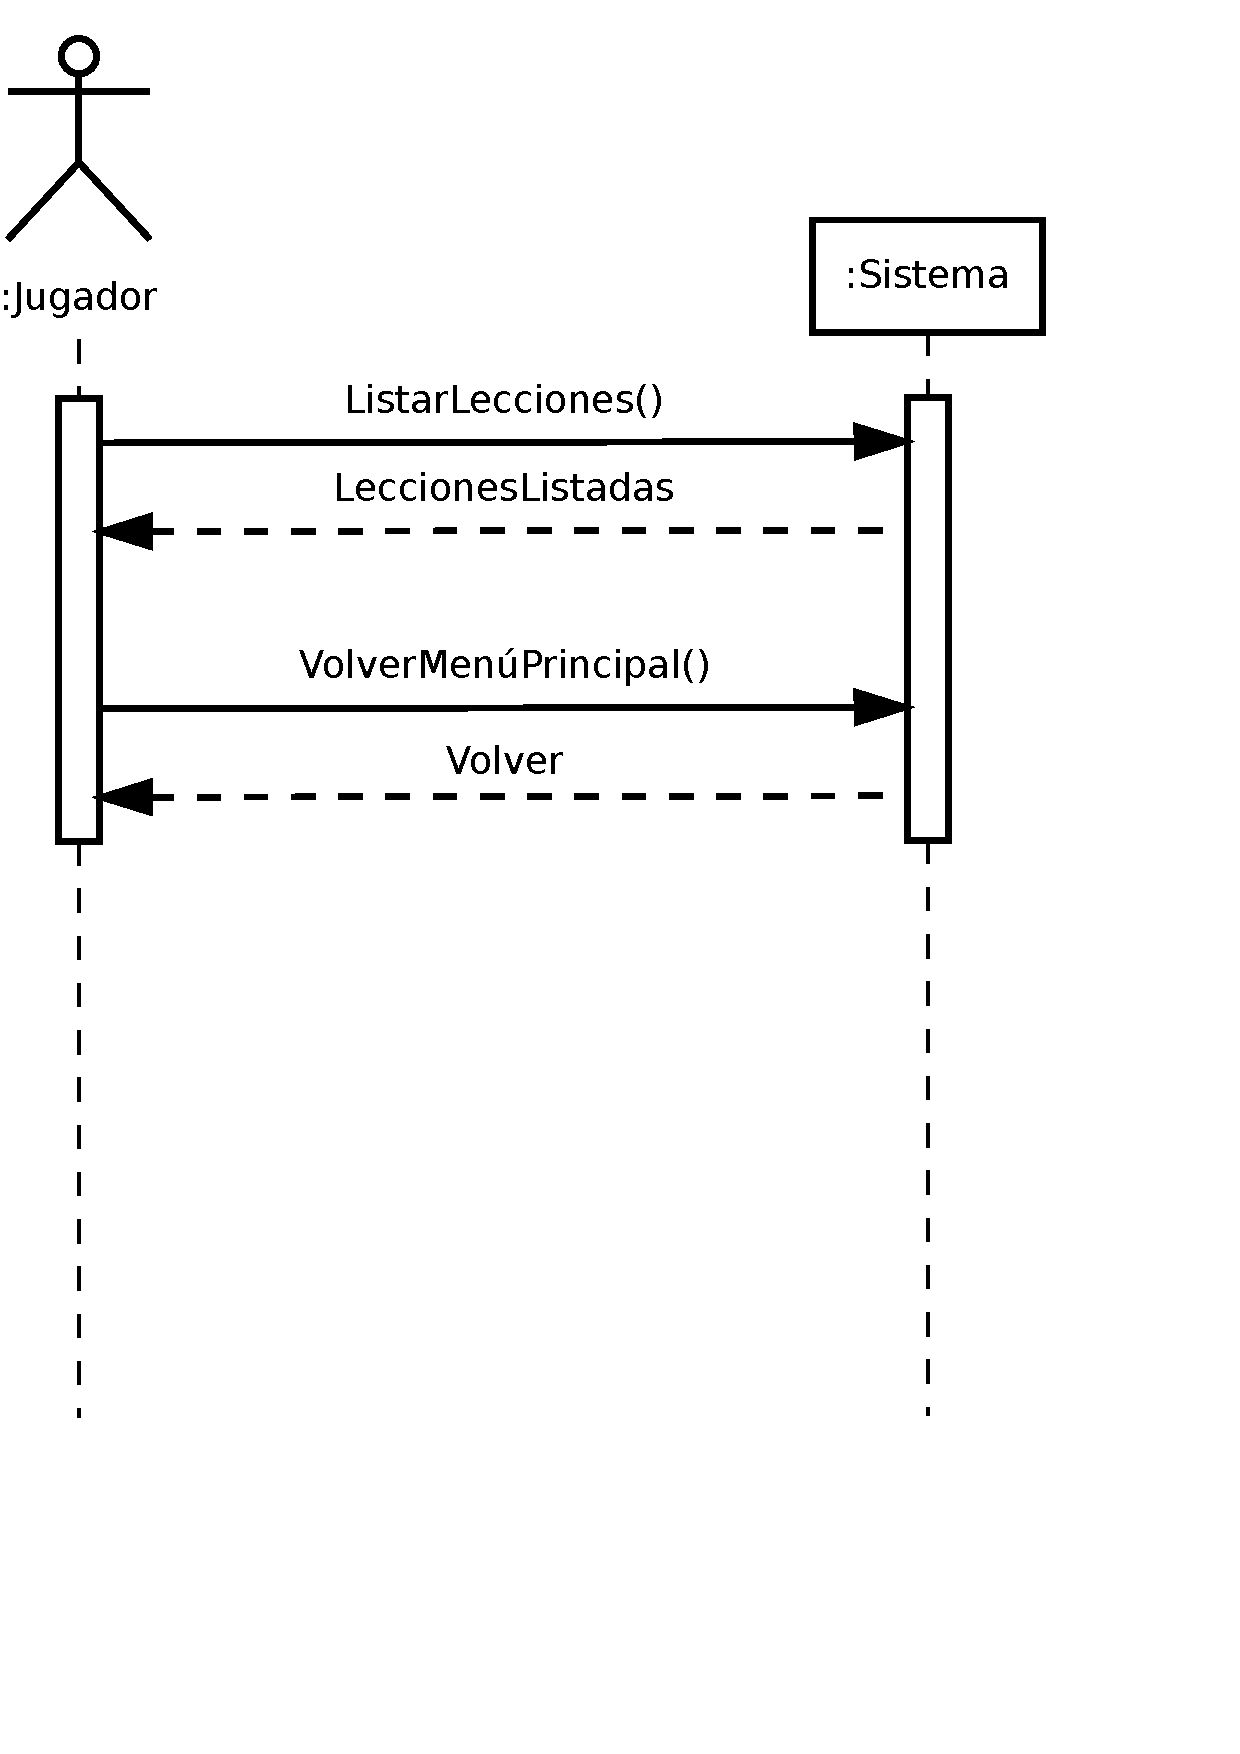
\includegraphics[trim=0cm 12cm 0cm 0cm, clip=true, width=0.5\textwidth]{4_analisis/diagsec_caso7_esc2}
  \caption{Diagrama de secuencia, selección de lecciones, escenario alternativo}
\end{figure}

\begin{description}
\item[Operación] ListarLecciones()
\item[Actores] \jugador\, \sistema\
\item[Responsabilidades] Mostrar el menú de selección de lecciones y listar
  todas las lecciones disponibles.
\item[Precondiciones] El usuario eligió la opción \textit{Lecciones} en el menú
  principal.
\item[Postcondiciones] $\quad$
  \begin{itemize}
  \item Se muestra la interfaz del menú de selección de lecciones.
  \item Se listan las lecciones cargadas en el sistema
  \end{itemize}
\end{description}

\begin{description}
\item[Operación] VolverMenuPrincipal()
\item[Actores] \jugador\, \sistema\
\item[Responsabilidades] Descargar el menú de selección de lecciones y volver al
  menú principal.
\item[Precondiciones] El usuario ha pulsado la tecla \texttt{escape} o el botón \textit{volver}.
\item[Postcondiciones] $\quad$
  \begin{itemize}
  \item Se descarga el menú de selección de lecciones.
  \item Se carga y muestra el menú principal
  \end{itemize}
\end{description}

%%% Local Variables: 
%%% mode: latex
%%% TeX-master: "../memoria"
%%% End: 

%%% Local Variables: 
%%% mode: latex
%%% TeX-master: "../memoria"
%%% End: 
